\chapter{Esempi su reti reali}
\section{Minnesota}
In questa sezione, andremo a simulare un epidemia su una rete reale: la rete stradale del Minnesota in Figura~\ref{fig::minesota}.\\
Per prima cosa abbiamo indagato come  i tassi d'infezione e di recupero modifichino la stiffness (vedi~\ref{stiff}) del modello chiuso alle coppie e alle triple.\\
Per indagare ci\`o abbiamo fatto variare i parametri di $\tau$ e $\gamma$ e abbiamo confrontato il numero d'iterazione delle funzioni ode45 e ode15s (Figura~\ref{fig::minnesota_lenght}). Per tutti i parametri la funzione ode15s impiega molte meno iterazioni, dunque il modello \`e stiff. Un'altra conferma di ci\`o ci viene dato anche calcolando il rapporto di stiff (Figura~\ref{fig::minnesota_ratiostiff}).\\ \\ 

Ci siamo anche chiesti come variasse la prevalenza, cambiando le condizioni inziali. In Figura~\ref{fig::minnesota_prevalenza} si osserva come, aumentando il grado del nodo in cui ``parte" l'epidemia, si velocizza il tempo per arrivare al picco. Inoltre notiamo che il picco rimane pressappoco uguale sia che si scelga un nodo di grado $1$ che uno di grado $5$ 
\begin{figure}[htb]
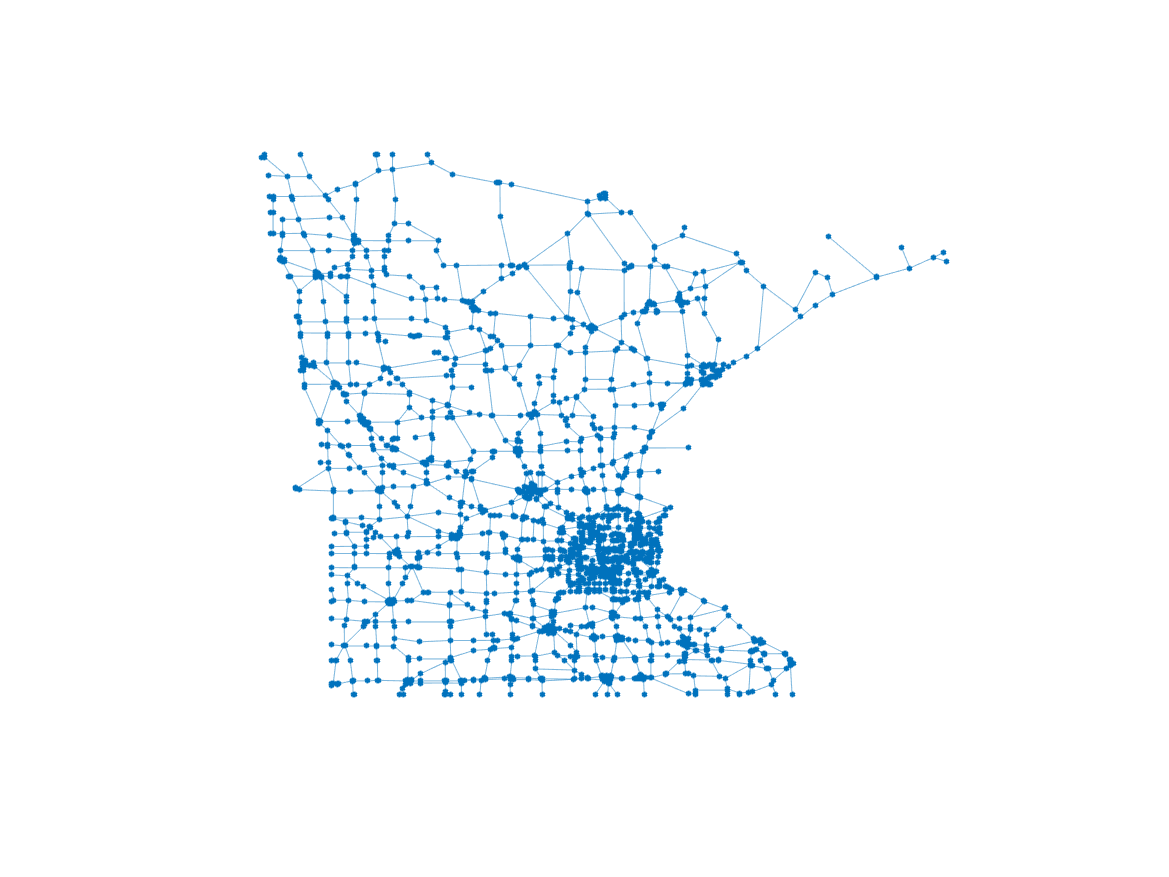
\includegraphics[scale=0.8]{Figure/minnesota}
	\caption{Grafico della rete stradale del Minnesota}
	\label{fig::minnesota}
\end{figure}
\begin{figure}[ht]
\centering
\subfloat[][$\gamma=0.10$]
{\resizebox{0.45\textwidth}{!}{% This file was created by matlab2tikz.
%
%The latest updates can be retrieved from
%  http://www.mathworks.com/matlabcentral/fileexchange/22022-matlab2tikz-matlab2tikz
%where you can also make suggestions and rate matlab2tikz.
%
\definecolor{mycolor1}{rgb}{0.00000,0.44700,0.74100}%
\definecolor{mycolor2}{rgb}{0.85000,0.32500,0.09800}%
%
\begin{tikzpicture}

\begin{axis}[%
width=0.39\columnwidth,
height=1.7in,
at={(1.011in,0.642in)},
scale only axis,
xmin=0,
xmax=1,
xlabel style={font=\color{white!15!black}},
xlabel={$\tau$},
ymin=0,
ymax=16000,
axis background/.style={fill=white},
legend columns=2,
legend pos=north west,
legend style={legend cell align=left, align=left, draw=none,fill=none}
]
\addplot [color=mycolor1, line width=2.0pt]
  table[row sep=crcr]{%
0	693\\
0.00252525252525253	693\\
0.00505050505050505	693\\
0.00757575757575758	693\\
0.0101010101010101	693\\
0.0126262626262626	693\\
0.0151515151515152	693\\
0.0176767676767677	693\\
0.0202020202020202	697\\
0.0227272727272727	701\\
0.0252525252525253	709\\
0.0277777777777778	717\\
0.0303030303030303	725\\
0.0328282828282828	733\\
0.0353535353535354	741\\
0.0378787878787879	749\\
0.0404040404040404	757\\
0.0429292929292929	765\\
0.0454545454545455	773\\
0.047979797979798	781\\
0.0505050505050505	785\\
0.053030303030303	793\\
0.0555555555555556	801\\
0.0580808080808081	809\\
0.0606060606060606	813\\
0.0631313131313131	821\\
0.0656565656565657	829\\
0.0681818181818182	833\\
0.0707070707070707	841\\
0.0732323232323232	845\\
0.0757575757575758	853\\
0.0782828282828283	861\\
0.0808080808080808	869\\
0.0833333333333333	881\\
0.0858585858585859	897\\
0.0883838383838384	913\\
0.0909090909090909	933\\
0.0934343434343434	957\\
0.095959595959596	981\\
0.0984848484848485	1001\\
0.101010101010101	1025\\
0.103535353535354	1049\\
0.106060606060606	1077\\
0.108585858585859	1101\\
0.111111111111111	1125\\
0.113636363636364	1153\\
0.116161616161616	1177\\
0.118686868686869	1205\\
0.121212121212121	1233\\
0.123737373737374	1261\\
0.126262626262626	1289\\
0.128787878787879	1317\\
0.131313131313131	1349\\
0.133838383838384	1377\\
0.136363636363636	1409\\
0.138888888888889	1441\\
0.141414141414141	1473\\
0.143939393939394	1505\\
0.146464646464646	1537\\
0.148989898989899	1569\\
0.151515151515152	1605\\
0.154040404040404	1637\\
0.156565656565657	1669\\
0.159090909090909	1701\\
0.161616161616162	1733\\
0.164141414141414	1765\\
0.166666666666667	1797\\
0.169191919191919	1829\\
0.171717171717172	1861\\
0.174242424242424	1897\\
0.176767676767677	1929\\
0.179292929292929	1961\\
0.181818181818182	1993\\
0.184343434343434	2029\\
0.186868686868687	2065\\
0.189393939393939	2097\\
0.191919191919192	2133\\
0.194444444444444	2165\\
0.196969696969697	2201\\
0.19949494949495	2237\\
0.202020202020202	2273\\
0.204545454545455	2309\\
0.207070707070707	2345\\
0.20959595959596	2381\\
0.212121212121212	2417\\
0.214646464646465	2453\\
0.217171717171717	2493\\
0.21969696969697	2533\\
0.222222222222222	2569\\
0.224747474747475	2609\\
0.227272727272727	2645\\
0.22979797979798	2685\\
0.232323232323232	2721\\
0.234848484848485	2757\\
0.237373737373737	2793\\
0.23989898989899	2829\\
0.242424242424242	2869\\
0.244949494949495	2905\\
0.247474747474747	2945\\
0.25	2981\\
0.25	2981\\
0.252525252525253	3017\\
0.255050505050505	3053\\
0.257575757575758	3093\\
0.26010101010101	3133\\
0.262626262626263	3173\\
0.265151515151515	3213\\
0.267676767676768	3253\\
0.27020202020202	3293\\
0.272727272727273	3333\\
0.275252525252525	3373\\
0.277777777777778	3413\\
0.28030303030303	3449\\
0.282828282828283	3489\\
0.285353535353535	3529\\
0.287878787878788	3569\\
0.29040404040404	3609\\
0.292929292929293	3649\\
0.295454545454545	3689\\
0.297979797979798	3729\\
0.30050505050505	3769\\
0.303030303030303	3809\\
0.305555555555556	3849\\
0.308080808080808	3889\\
0.310606060606061	3929\\
0.313131313131313	3969\\
0.315656565656566	4009\\
0.318181818181818	4045\\
0.320707070707071	4085\\
0.323232323232323	4125\\
0.325757575757576	4165\\
0.328282828282828	4205\\
0.330808080808081	4245\\
0.333333333333333	4281\\
0.335858585858586	4321\\
0.338383838383838	4361\\
0.340909090909091	4397\\
0.343434343434343	4437\\
0.345959595959596	4481\\
0.348484848484849	4525\\
0.351010101010101	4565\\
0.353535353535354	4609\\
0.356060606060606	4649\\
0.358585858585859	4689\\
0.361111111111111	4729\\
0.363636363636364	4769\\
0.366161616161616	4809\\
0.368686868686869	4849\\
0.371212121212121	4889\\
0.373737373737374	4929\\
0.376262626262626	4973\\
0.378787878787879	5013\\
0.381313131313131	5053\\
0.383838383838384	5093\\
0.386363636363636	5137\\
0.388888888888889	5177\\
0.391414141414141	5217\\
0.393939393939394	5257\\
0.396464646464646	5297\\
0.398989898989899	5341\\
0.401515151515151	5381\\
0.404040404040404	5421\\
0.406565656565657	5461\\
0.409090909090909	5501\\
0.411616161616162	5541\\
0.414141414141414	5581\\
0.416666666666667	5621\\
0.419191919191919	5661\\
0.421717171717172	5705\\
0.424242424242424	5745\\
0.426767676767677	5785\\
0.429292929292929	5825\\
0.431818181818182	5869\\
0.434343434343434	5909\\
0.436868686868687	5949\\
0.439393939393939	5993\\
0.441919191919192	6037\\
0.444444444444444	6077\\
0.446969696969697	6121\\
0.44949494949495	6161\\
0.452020202020202	6205\\
0.454545454545455	6249\\
0.457070707070707	6289\\
0.45959595959596	6333\\
0.462121212121212	6373\\
0.464646464646465	6413\\
0.467171717171717	6453\\
0.46969696969697	6497\\
0.472222222222222	6537\\
0.474747474747475	6581\\
0.477272727272727	6625\\
0.47979797979798	6669\\
0.482323232323232	6713\\
0.484848484848485	6753\\
0.487373737373737	6797\\
0.48989898989899	6841\\
0.492424242424242	6885\\
0.494949494949495	6929\\
0.497474747474748	6977\\
0.5	7021\\
0.5	7021\\
0.502525252525252	7061\\
0.505050505050505	7105\\
0.507575757575758	7149\\
0.51010101010101	7189\\
0.512626262626263	7233\\
0.515151515151515	7273\\
0.517676767676768	7317\\
0.52020202020202	7361\\
0.522727272727273	7401\\
0.525252525252525	7445\\
0.527777777777778	7485\\
0.53030303030303	7529\\
0.532828282828283	7569\\
0.535353535353535	7613\\
0.537878787878788	7653\\
0.54040404040404	7697\\
0.542929292929293	7741\\
0.545454545454545	7781\\
0.547979797979798	7825\\
0.55050505050505	7865\\
0.553030303030303	7909\\
0.555555555555556	7953\\
0.558080808080808	7997\\
0.560606060606061	8041\\
0.563131313131313	8085\\
0.565656565656566	8129\\
0.568181818181818	8169\\
0.570707070707071	8213\\
0.573232323232323	8253\\
0.575757575757576	8293\\
0.578282828282828	8337\\
0.580808080808081	8377\\
0.583333333333333	8417\\
0.585858585858586	8457\\
0.588383838383838	8501\\
0.590909090909091	8541\\
0.593434343434343	8585\\
0.595959595959596	8629\\
0.598484848484849	8669\\
0.601010101010101	8713\\
0.603535353535354	8757\\
0.606060606060606	8801\\
0.608585858585859	8845\\
0.611111111111111	8885\\
0.613636363636364	8929\\
0.616161616161616	8977\\
0.618686868686869	9021\\
0.621212121212121	9065\\
0.623737373737374	9109\\
0.626262626262626	9153\\
0.628787878787879	9197\\
0.631313131313131	9241\\
0.633838383838384	9285\\
0.636363636363636	9329\\
0.638888888888889	9369\\
0.641414141414141	9413\\
0.643939393939394	9457\\
0.646464646464646	9501\\
0.648989898989899	9545\\
0.651515151515151	9589\\
0.654040404040404	9633\\
0.656565656565657	9677\\
0.659090909090909	9721\\
0.661616161616162	9765\\
0.664141414141414	9809\\
0.666666666666667	9853\\
0.669191919191919	9897\\
0.671717171717172	9945\\
0.674242424242424	9989\\
0.676767676767677	10037\\
0.679292929292929	10081\\
0.681818181818182	10125\\
0.684343434343434	10169\\
0.686868686868687	10213\\
0.689393939393939	10257\\
0.691919191919192	10297\\
0.694444444444444	10341\\
0.696969696969697	10381\\
0.69949494949495	10425\\
0.702020202020202	10469\\
0.704545454545455	10509\\
0.707070707070707	10553\\
0.70959595959596	10597\\
0.712121212121212	10641\\
0.714646464646465	10681\\
0.717171717171717	10725\\
0.71969696969697	10773\\
0.722222222222222	10817\\
0.724747474747475	10861\\
0.727272727272727	10905\\
0.72979797979798	10953\\
0.732323232323232	10997\\
0.734848484848485	11041\\
0.737373737373737	11085\\
0.73989898989899	11133\\
0.742424242424242	11177\\
0.744949494949495	11221\\
0.747474747474748	11265\\
0.75	11309\\
0.75	11309\\
0.752525252525252	11353\\
0.755050505050505	11397\\
0.757575757575758	11441\\
0.76010101010101	11481\\
0.762626262626263	11525\\
0.765151515151515	11565\\
0.767676767676768	11613\\
0.77020202020202	11657\\
0.772727272727273	11705\\
0.775252525252525	11749\\
0.777777777777778	11797\\
0.78030303030303	11841\\
0.782828282828283	11889\\
0.785353535353535	11933\\
0.787878787878788	11977\\
0.79040404040404	12021\\
0.792929292929293	12065\\
0.795454545454545	12109\\
0.797979797979798	12153\\
0.80050505050505	12193\\
0.803030303030303	12233\\
0.805555555555556	12277\\
0.808080808080808	12317\\
0.810606060606061	12357\\
0.813131313131313	12401\\
0.815656565656566	12441\\
0.818181818181818	12485\\
0.820707070707071	12529\\
0.823232323232323	12577\\
0.825757575757576	12621\\
0.828282828282828	12669\\
0.830808080808081	12713\\
0.833333333333333	12761\\
0.835858585858586	12805\\
0.838383838383838	12853\\
0.840909090909091	12897\\
0.843434343434343	12941\\
0.845959595959596	12985\\
0.848484848484849	13029\\
0.851010101010101	13073\\
0.853535353535354	13117\\
0.856060606060606	13161\\
0.858585858585859	13201\\
0.861111111111111	13241\\
0.863636363636364	13281\\
0.866161616161616	13321\\
0.868686868686869	13361\\
0.871212121212121	13397\\
0.873737373737374	13437\\
0.876262626262626	13477\\
0.878787878787879	13517\\
0.881313131313131	13557\\
0.883838383838384	13601\\
0.886363636363636	13645\\
0.888888888888889	13693\\
0.891414141414141	13737\\
0.893939393939394	13781\\
0.896464646464646	13825\\
0.898989898989899	13873\\
0.901515151515151	13917\\
0.904040404040404	13957\\
0.906565656565657	14001\\
0.909090909090909	14041\\
0.911616161616162	14081\\
0.914141414141414	14121\\
0.916666666666667	14161\\
0.919191919191919	14197\\
0.921717171717172	14237\\
0.924242424242424	14277\\
0.926767676767677	14317\\
0.929292929292929	14357\\
0.931818181818182	14401\\
0.934343434343434	14445\\
0.936868686868687	14489\\
0.939393939393939	14533\\
0.941919191919192	14577\\
0.944444444444444	14617\\
0.946969696969697	14661\\
0.94949494949495	14701\\
0.952020202020202	14741\\
0.954545454545455	14781\\
0.957070707070707	14821\\
0.95959595959596	14861\\
0.962121212121212	14897\\
0.964646464646465	14937\\
0.967171717171717	14973\\
0.96969696969697	15013\\
0.972222222222222	15049\\
0.974747474747475	15085\\
0.977272727272727	15125\\
0.97979797979798	15165\\
0.982323232323232	15205\\
0.984848484848485	15245\\
0.987373737373737	15285\\
0.98989898989899	15325\\
0.992424242424242	15365\\
0.994949494949495	15405\\
0.997474747474748	15445\\
1	15485\\
};
\addlegendentry{ode45}

\addplot [color=mycolor2, line width=2.0pt]
  table[row sep=crcr]{%
0	253\\
0.00252525252525253	253\\
0.00505050505050505	253\\
0.00757575757575758	253\\
0.0101010101010101	253\\
0.0126262626262626	255\\
0.0151515151515152	259\\
0.0176767676767677	265\\
0.0202020202020202	271\\
0.0227272727272727	277\\
0.0252525252525253	282\\
0.0277777777777778	288\\
0.0303030303030303	295\\
0.0328282828282828	300\\
0.0353535353535354	305\\
0.0378787878787879	311\\
0.0404040404040404	312\\
0.0429292929292929	320\\
0.0454545454545455	324\\
0.047979797979798	329\\
0.0505050505050505	333\\
0.053030303030303	338\\
0.0555555555555556	342\\
0.0580808080808081	346\\
0.0606060606060606	350\\
0.0631313131313131	354\\
0.0656565656565657	358\\
0.0681818181818182	361\\
0.0707070707070707	365\\
0.0732323232323232	369\\
0.0757575757575758	373\\
0.0782828282828283	380\\
0.0808080808080808	387\\
0.0833333333333333	395\\
0.0858585858585859	403\\
0.0883838383838384	415\\
0.0909090909090909	424\\
0.0934343434343434	434\\
0.095959595959596	443\\
0.0984848484848485	454\\
0.101010101010101	464\\
0.103535353535354	475\\
0.106060606060606	486\\
0.108585858585859	497\\
0.111111111111111	509\\
0.113636363636364	522\\
0.116161616161616	529\\
0.118686868686869	543\\
0.121212121212121	557\\
0.123737373737374	574\\
0.126262626262626	588\\
0.128787878787879	597\\
0.131313131313131	611\\
0.133838383838384	625\\
0.136363636363636	638\\
0.138888888888889	652\\
0.141414141414141	665\\
0.143939393939394	679\\
0.146464646464646	692\\
0.148989898989899	706\\
0.151515151515152	719\\
0.154040404040404	732\\
0.156565656565657	745\\
0.159090909090909	759\\
0.161616161616162	773\\
0.164141414141414	786\\
0.166666666666667	800\\
0.169191919191919	813\\
0.171717171717172	826\\
0.174242424242424	840\\
0.176767676767677	853\\
0.179292929292929	866\\
0.181818181818182	880\\
0.184343434343434	894\\
0.186868686868687	908\\
0.189393939393939	922\\
0.191919191919192	935\\
0.194444444444444	949\\
0.196969696969697	962\\
0.19949494949495	976\\
0.202020202020202	989\\
0.204545454545455	1002\\
0.207070707070707	1017\\
0.20959595959596	1031\\
0.212121212121212	1044\\
0.214646464646465	1059\\
0.217171717171717	1072\\
0.21969696969697	1088\\
0.222222222222222	1099\\
0.224747474747475	1115\\
0.227272727272727	1128\\
0.22979797979798	1145\\
0.232323232323232	1157\\
0.234848484848485	1169\\
0.237373737373737	1186\\
0.23989898989899	1204\\
0.242424242424242	1219\\
0.244949494949495	1236\\
0.247474747474747	1252\\
0.25	1272\\
0.25	1272\\
0.252525252525253	1289\\
0.255050505050505	1302\\
0.257575757575758	1319\\
0.26010101010101	1335\\
0.262626262626263	1351\\
0.265151515151515	1366\\
0.267676767676768	1380\\
0.27020202020202	1395\\
0.272727272727273	1409\\
0.275252525252525	1424\\
0.277777777777778	1439\\
0.28030303030303	1453\\
0.282828282828283	1467\\
0.285353535353535	1481\\
0.287878787878788	1496\\
0.29040404040404	1511\\
0.292929292929293	1526\\
0.295454545454545	1541\\
0.297979797979798	1555\\
0.30050505050505	1570\\
0.303030303030303	1585\\
0.305555555555556	1600\\
0.308080808080808	1614\\
0.310606060606061	1629\\
0.313131313131313	1644\\
0.315656565656566	1660\\
0.318181818181818	1675\\
0.320707070707071	1693\\
0.323232323232323	1711\\
0.325757575757576	1729\\
0.328282828282828	1745\\
0.330808080808081	1762\\
0.333333333333333	1779\\
0.335858585858586	1794\\
0.338383838383838	1810\\
0.340909090909091	1825\\
0.343434343434343	1844\\
0.345959595959596	1860\\
0.348484848484849	1876\\
0.351010101010101	1890\\
0.353535353535354	1907\\
0.356060606060606	1922\\
0.358585858585859	1938\\
0.361111111111111	1953\\
0.363636363636364	1970\\
0.366161616161616	1988\\
0.368686868686869	2005\\
0.371212121212121	2021\\
0.373737373737374	2033\\
0.376262626262626	2051\\
0.378787878787879	2067\\
0.381313131313131	2083\\
0.383838383838384	2099\\
0.386363636363636	2114\\
0.388888888888889	2130\\
0.391414141414141	2144\\
0.393939393939394	2160\\
0.396464646464646	2176\\
0.398989898989899	2194\\
0.401515151515151	2207\\
0.404040404040404	2222\\
0.406565656565657	2239\\
0.409090909090909	2255\\
0.411616161616162	2271\\
0.414141414141414	2287\\
0.416666666666667	2304\\
0.419191919191919	2317\\
0.421717171717172	2332\\
0.424242424242424	2349\\
0.426767676767677	2365\\
0.429292929292929	2381\\
0.431818181818182	2398\\
0.434343434343434	2410\\
0.436868686868687	2424\\
0.439393939393939	2438\\
0.441919191919192	2453\\
0.444444444444444	2471\\
0.446969696969697	2493\\
0.44949494949495	2519\\
0.452020202020202	2532\\
0.454545454545455	2542\\
0.457070707070707	2559\\
0.45959595959596	2577\\
0.462121212121212	2596\\
0.464646464646465	2613\\
0.467171717171717	2628\\
0.46969696969697	2655\\
0.472222222222222	2670\\
0.474747474747475	2682\\
0.477272727272727	2698\\
0.47979797979798	2715\\
0.482323232323232	2732\\
0.484848484848485	2745\\
0.487373737373737	2757\\
0.48989898989899	2776\\
0.492424242424242	2792\\
0.494949494949495	2827\\
0.497474747474748	2844\\
0.5	2848\\
0.5	2848\\
0.502525252525252	2865\\
0.505050505050505	2881\\
0.507575757575758	2896\\
0.51010101010101	2917\\
0.512626262626263	2933\\
0.515151515151515	2946\\
0.517676767676768	2964\\
0.52020202020202	2979\\
0.522727272727273	2997\\
0.525252525252525	3014\\
0.527777777777778	3028\\
0.53030303030303	3048\\
0.532828282828283	3063\\
0.535353535353535	3081\\
0.537878787878788	3097\\
0.54040404040404	3114\\
0.542929292929293	3126\\
0.545454545454545	3143\\
0.547979797979798	3159\\
0.55050505050505	3175\\
0.553030303030303	3193\\
0.555555555555556	3211\\
0.558080808080808	3227\\
0.560606060606061	3244\\
0.563131313131313	3262\\
0.565656565656566	3269\\
0.568181818181818	3283\\
0.570707070707071	3301\\
0.573232323232323	3328\\
0.575757575757576	3340\\
0.578282828282828	3357\\
0.580808080808081	3374\\
0.583333333333333	3391\\
0.585858585858586	3418\\
0.588383838383838	3430\\
0.590909090909091	3443\\
0.593434343434343	3460\\
0.595959595959596	3474\\
0.598484848484849	3495\\
0.601010101010101	3512\\
0.603535353535354	3529\\
0.606060606060606	3540\\
0.608585858585859	3561\\
0.611111111111111	3573\\
0.613636363636364	3595\\
0.616161616161616	3611\\
0.618686868686869	3627\\
0.621212121212121	3643\\
0.623737373737374	3659\\
0.626262626262626	3680\\
0.628787878787879	3703\\
0.631313131313131	3719\\
0.633838383838384	3741\\
0.636363636363636	3755\\
0.638888888888889	3771\\
0.641414141414141	3790\\
0.643939393939394	3812\\
0.646464646464646	3825\\
0.648989898989899	3843\\
0.651515151515151	3864\\
0.654040404040404	3883\\
0.656565656565657	3901\\
0.659090909090909	3918\\
0.661616161616162	3932\\
0.664141414141414	3951\\
0.666666666666667	3967\\
0.669191919191919	3985\\
0.671717171717172	4004\\
0.674242424242424	4024\\
0.676767676767677	4043\\
0.679292929292929	4062\\
0.681818181818182	4081\\
0.684343434343434	4099\\
0.686868686868687	4112\\
0.689393939393939	4132\\
0.691919191919192	4144\\
0.694444444444444	4151\\
0.696969696969697	4168\\
0.69949494949495	4198\\
0.702020202020202	4210\\
0.704545454545455	4225\\
0.707070707070707	4239\\
0.70959595959596	4254\\
0.712121212121212	4271\\
0.714646464646465	4286\\
0.717171717171717	4303\\
0.71969696969697	4317\\
0.722222222222222	4337\\
0.724747474747475	4357\\
0.727272727272727	4374\\
0.72979797979798	4392\\
0.732323232323232	4412\\
0.734848484848485	4431\\
0.737373737373737	4447\\
0.73989898989899	4467\\
0.742424242424242	4487\\
0.744949494949495	4506\\
0.747474747474748	4523\\
0.75	4542\\
0.75	4542\\
0.752525252525252	4560\\
0.755050505050505	4576\\
0.757575757575758	4599\\
0.76010101010101	4625\\
0.762626262626263	4646\\
0.765151515151515	4675\\
0.767676767676768	4711\\
0.77020202020202	4754\\
0.772727272727273	4809\\
0.775252525252525	4875\\
0.777777777777778	4968\\
0.78030303030303	5101\\
0.782828282828283	5423\\
0.785353535353535	10728\\
0.787878787878788	10726\\
0.79040404040404	10725\\
0.792929292929293	10722\\
0.795454545454545	10719\\
0.797979797979798	10718\\
0.80050505050505	10716\\
0.803030303030303	10711\\
0.805555555555556	10712\\
0.808080808080808	10710\\
0.810606060606061	10708\\
0.813131313131313	10706\\
0.815656565656566	10706\\
0.818181818181818	10704\\
0.820707070707071	10703\\
0.823232323232323	10700\\
0.825757575757576	10700\\
0.828282828282828	10698\\
0.830808080808081	10697\\
0.833333333333333	10695\\
0.835858585858586	10696\\
0.838383838383838	10694\\
0.840909090909091	10693\\
0.843434343434343	10691\\
0.845959595959596	10693\\
0.848484848484849	10687\\
0.851010101010101	10690\\
0.853535353535354	10685\\
0.856060606060606	10686\\
0.858585858585859	10685\\
0.861111111111111	10685\\
0.863636363636364	10681\\
0.866161616161616	10684\\
0.868686868686869	10678\\
0.871212121212121	5339\\
0.873737373737374	5357\\
0.876262626262626	5376\\
0.878787878787879	5391\\
0.881313131313131	5401\\
0.883838383838384	5423\\
0.886363636363636	10925\\
0.888888888888889	10964\\
0.891414141414141	10950\\
0.893939393939394	10966\\
0.896464646464646	10953\\
0.898989898989899	10972\\
0.901515151515151	10956\\
0.904040404040404	11030\\
0.906565656565657	10961\\
0.909090909090909	11042\\
0.911616161616162	11019\\
0.914141414141414	10951\\
0.916666666666667	11032\\
0.919191919191919	11010\\
0.921717171717172	10950\\
0.924242424242424	11021\\
0.926767676767677	10998\\
0.929292929292929	10980\\
0.931818181818182	10931\\
0.934343434343434	10974\\
0.936868686868687	10977\\
0.939393939393939	10928\\
0.941919191919192	10915\\
0.944444444444444	10952\\
0.946969696969697	10940\\
0.94949494949495	10898\\
0.952020202020202	10940\\
0.954545454545455	10931\\
0.957070707070707	10920\\
0.95959595959596	10884\\
0.962121212121212	10879\\
0.964646464646465	10906\\
0.967171717171717	10894\\
0.96969696969697	10886\\
0.972222222222222	10870\\
0.974747474747475	10866\\
0.977272727272727	10884\\
0.97979797979798	10879\\
0.982323232323232	10875\\
0.984848484848485	10849\\
0.987373737373737	10845\\
0.98989898989899	10875\\
0.992424242424242	10872\\
0.994949494949495	10866\\
0.997474747474748	10842\\
1	10845\\
};
\addlegendentry{ode15s}
\end{axis}
\end{tikzpicture}%}}
 \quad 
\subfloat[][$\gamma=0.30$]
{\resizebox{0.45\textwidth}{!}{ % This file was created by matlab2tikz.
%
%The latest updates can be retrieved from
%  http://www.mathworks.com/matlabcentral/fileexchange/22022-matlab2tikz-matlab2tikz
%where you can also make suggestions and rate matlab2tikz.
%
\definecolor{mycolor1}{rgb}{0.00000,0.44700,0.74100}%
\definecolor{mycolor2}{rgb}{0.85000,0.32500,0.09800}%
%
\begin{tikzpicture}

\begin{axis}[%
width=6.028in,
height=4.754in,
at={(1.011in,0.642in)},
scale only axis,
xmin=0,
xmax=1,
xlabel style={font=\color{white!15!black}},
xlabel={$\tau$},
ymin=0,
ymax=14000,
ylabel style={font=\color{white!15!black}},
ylabel={iterazioni},
axis background/.style={fill=white},
legend style={legend cell align=left, align=left, draw=white!15!black}
]
\addplot [color=mycolor1, line width=2.0pt]
  table[row sep=crcr]{%
0	1281\\
0.00252525252525253	1281\\
0.00505050505050505	1281\\
0.00757575757575758	1281\\
0.0101010101010101	1281\\
0.0126262626262626	1281\\
0.0151515151515152	1281\\
0.0176767676767677	1281\\
0.0202020202020202	1281\\
0.0227272727272727	1281\\
0.0252525252525253	1281\\
0.0277777777777778	1281\\
0.0303030303030303	1281\\
0.0328282828282828	1281\\
0.0353535353535354	1281\\
0.0378787878787879	1281\\
0.0404040404040404	1281\\
0.0429292929292929	1281\\
0.0454545454545455	1281\\
0.047979797979798	1281\\
0.0505050505050505	1281\\
0.053030303030303	1281\\
0.0555555555555556	1281\\
0.0580808080808081	1285\\
0.0606060606060606	1285\\
0.0631313131313131	1289\\
0.0656565656565657	1289\\
0.0681818181818182	1293\\
0.0707070707070707	1293\\
0.0732323232323232	1297\\
0.0757575757575758	1297\\
0.0782828282828283	1301\\
0.0808080808080808	1305\\
0.0833333333333333	1305\\
0.0858585858585859	1309\\
0.0883838383838384	1309\\
0.0909090909090909	1313\\
0.0934343434343434	1317\\
0.095959595959596	1317\\
0.0984848484848485	1321\\
0.101010101010101	1325\\
0.103535353535354	1325\\
0.106060606060606	1329\\
0.108585858585859	1333\\
0.111111111111111	1333\\
0.113636363636364	1337\\
0.116161616161616	1341\\
0.118686868686869	1341\\
0.121212121212121	1345\\
0.123737373737374	1349\\
0.126262626262626	1349\\
0.128787878787879	1353\\
0.131313131313131	1357\\
0.133838383838384	1357\\
0.136363636363636	1361\\
0.138888888888889	1365\\
0.141414141414141	1365\\
0.143939393939394	1369\\
0.146464646464646	1373\\
0.148989898989899	1381\\
0.151515151515152	1389\\
0.154040404040404	1397\\
0.156565656565657	1405\\
0.159090909090909	1413\\
0.161616161616162	1425\\
0.164141414141414	1433\\
0.166666666666667	1445\\
0.169191919191919	1457\\
0.171717171717172	1473\\
0.174242424242424	1485\\
0.176767676767677	1497\\
0.179292929292929	1513\\
0.181818181818182	1529\\
0.184343434343434	1541\\
0.186868686868687	1557\\
0.189393939393939	1573\\
0.191919191919192	1589\\
0.194444444444444	1605\\
0.196969696969697	1621\\
0.19949494949495	1637\\
0.202020202020202	1653\\
0.204545454545455	1673\\
0.207070707070707	1689\\
0.20959595959596	1709\\
0.212121212121212	1729\\
0.214646464646465	1749\\
0.217171717171717	1773\\
0.21969696969697	1793\\
0.222222222222222	1817\\
0.224747474747475	1837\\
0.227272727272727	1861\\
0.22979797979798	1885\\
0.232323232323232	1909\\
0.234848484848485	1933\\
0.237373737373737	1957\\
0.23989898989899	1981\\
0.242424242424242	2005\\
0.244949494949495	2029\\
0.247474747474747	2057\\
0.25	2081\\
0.25	2081\\
0.252525252525253	2109\\
0.255050505050505	2137\\
0.257575757575758	2169\\
0.26010101010101	2197\\
0.262626262626263	2229\\
0.265151515151515	2261\\
0.267676767676768	2293\\
0.27020202020202	2321\\
0.272727272727273	2353\\
0.275252525252525	2381\\
0.277777777777778	2413\\
0.28030303030303	2441\\
0.282828282828283	2469\\
0.285353535353535	2501\\
0.287878787878788	2529\\
0.29040404040404	2561\\
0.292929292929293	2589\\
0.295454545454545	2621\\
0.297979797979798	2653\\
0.30050505050505	2681\\
0.303030303030303	2713\\
0.305555555555556	2741\\
0.308080808080808	2773\\
0.310606060606061	2805\\
0.313131313131313	2837\\
0.315656565656566	2865\\
0.318181818181818	2897\\
0.320707070707071	2929\\
0.323232323232323	2961\\
0.325757575757576	2993\\
0.328282828282828	3021\\
0.330808080808081	3053\\
0.333333333333333	3085\\
0.335858585858586	3117\\
0.338383838383838	3153\\
0.340909090909091	3185\\
0.343434343434343	3221\\
0.345959595959596	3257\\
0.348484848484849	3293\\
0.351010101010101	3329\\
0.353535353535354	3365\\
0.356060606060606	3401\\
0.358585858585859	3433\\
0.361111111111111	3465\\
0.363636363636364	3501\\
0.366161616161616	3533\\
0.368686868686869	3569\\
0.371212121212121	3601\\
0.373737373737374	3637\\
0.376262626262626	3673\\
0.378787878787879	3705\\
0.381313131313131	3741\\
0.383838383838384	3773\\
0.386363636363636	3809\\
0.388888888888889	3841\\
0.391414141414141	3873\\
0.393939393939394	3909\\
0.396464646464646	3941\\
0.398989898989899	3977\\
0.401515151515151	4009\\
0.404040404040404	4045\\
0.406565656565657	4077\\
0.409090909090909	4113\\
0.411616161616162	4145\\
0.414141414141414	4181\\
0.416666666666667	4213\\
0.419191919191919	4249\\
0.421717171717172	4285\\
0.424242424242424	4317\\
0.426767676767677	4353\\
0.429292929292929	4389\\
0.431818181818182	4425\\
0.434343434343434	4461\\
0.436868686868687	4497\\
0.439393939393939	4533\\
0.441919191919192	4569\\
0.444444444444444	4605\\
0.446969696969697	4641\\
0.44949494949495	4677\\
0.452020202020202	4709\\
0.454545454545455	4745\\
0.457070707070707	4781\\
0.45959595959596	4813\\
0.462121212121212	4849\\
0.464646464646465	4889\\
0.467171717171717	4925\\
0.46969696969697	4965\\
0.472222222222222	5001\\
0.474747474747475	5041\\
0.477272727272727	5081\\
0.47979797979798	5121\\
0.482323232323232	5157\\
0.484848484848485	5197\\
0.487373737373737	5237\\
0.48989898989899	5277\\
0.492424242424242	5317\\
0.494949494949495	5361\\
0.497474747474748	5401\\
0.5	5441\\
0.5	5441\\
0.502525252525252	5481\\
0.505050505050505	5521\\
0.507575757575758	5557\\
0.51010101010101	5593\\
0.512626262626263	5633\\
0.515151515151515	5669\\
0.517676767676768	5709\\
0.52020202020202	5745\\
0.522727272727273	5785\\
0.525252525252525	5821\\
0.527777777777778	5861\\
0.53030303030303	5897\\
0.532828282828283	5937\\
0.535353535353535	5973\\
0.537878787878788	6013\\
0.54040404040404	6053\\
0.542929292929293	6093\\
0.545454545454545	6129\\
0.547979797979798	6169\\
0.55050505050505	6209\\
0.553030303030303	6249\\
0.555555555555556	6289\\
0.558080808080808	6329\\
0.560606060606061	6369\\
0.563131313131313	6409\\
0.565656565656566	6445\\
0.568181818181818	6485\\
0.570707070707071	6521\\
0.573232323232323	6557\\
0.575757575757576	6597\\
0.578282828282828	6633\\
0.580808080808081	6669\\
0.583333333333333	6705\\
0.585858585858586	6745\\
0.588383838383838	6781\\
0.590909090909091	6821\\
0.593434343434343	6857\\
0.595959595959596	6893\\
0.598484848484849	6933\\
0.601010101010101	6973\\
0.603535353535354	7013\\
0.606060606060606	7049\\
0.608585858585859	7089\\
0.611111111111111	7129\\
0.613636363636364	7169\\
0.616161616161616	7209\\
0.618686868686869	7249\\
0.621212121212121	7289\\
0.623737373737374	7329\\
0.626262626262626	7373\\
0.628787878787879	7413\\
0.631313131313131	7453\\
0.633838383838384	7493\\
0.636363636363636	7533\\
0.638888888888889	7573\\
0.641414141414141	7613\\
0.643939393939394	7649\\
0.646464646464646	7689\\
0.648989898989899	7729\\
0.651515151515151	7769\\
0.654040404040404	7813\\
0.656565656565657	7853\\
0.659090909090909	7893\\
0.661616161616162	7933\\
0.664141414141414	7973\\
0.666666666666667	8017\\
0.669191919191919	8061\\
0.671717171717172	8105\\
0.674242424242424	8149\\
0.676767676767677	8193\\
0.679292929292929	8237\\
0.681818181818182	8277\\
0.684343434343434	8321\\
0.686868686868687	8361\\
0.689393939393939	8401\\
0.691919191919192	8441\\
0.694444444444444	8481\\
0.696969696969697	8521\\
0.69949494949495	8561\\
0.702020202020202	8605\\
0.704545454545455	8645\\
0.707070707070707	8685\\
0.70959595959596	8725\\
0.712121212121212	8769\\
0.714646464646465	8809\\
0.717171717171717	8853\\
0.71969696969697	8897\\
0.722222222222222	8941\\
0.724747474747475	8981\\
0.727272727272727	9025\\
0.72979797979798	9069\\
0.732323232323232	9113\\
0.734848484848485	9157\\
0.737373737373737	9197\\
0.73989898989899	9241\\
0.742424242424242	9285\\
0.744949494949495	9325\\
0.747474747474748	9369\\
0.75	9409\\
0.75	9409\\
0.752525252525252	9453\\
0.755050505050505	9493\\
0.757575757575758	9533\\
0.76010101010101	9573\\
0.762626262626263	9617\\
0.765151515151515	9657\\
0.767676767676768	9701\\
0.77020202020202	9745\\
0.772727272727273	9785\\
0.775252525252525	9829\\
0.777777777777778	9873\\
0.78030303030303	9913\\
0.782828282828283	9957\\
0.785353535353535	10001\\
0.787878787878788	10041\\
0.79040404040404	10085\\
0.792929292929293	10125\\
0.795454545454545	10169\\
0.797979797979798	10209\\
0.80050505050505	10249\\
0.803030303030303	10293\\
0.805555555555556	10333\\
0.808080808080808	10373\\
0.810606060606061	10413\\
0.813131313131313	10457\\
0.815656565656566	10497\\
0.818181818181818	10541\\
0.820707070707071	10589\\
0.823232323232323	10633\\
0.825757575757576	10673\\
0.828282828282828	10721\\
0.830808080808081	10765\\
0.833333333333333	10809\\
0.835858585858586	10857\\
0.838383838383838	10901\\
0.840909090909091	10945\\
0.843434343434343	10989\\
0.845959595959596	11029\\
0.848484848484849	11073\\
0.851010101010101	11113\\
0.853535353535354	11153\\
0.856060606060606	11193\\
0.858585858585859	11233\\
0.861111111111111	11273\\
0.863636363636364	11313\\
0.866161616161616	11357\\
0.868686868686869	11401\\
0.871212121212121	11441\\
0.873737373737374	11489\\
0.876262626262626	11533\\
0.878787878787879	11577\\
0.881313131313131	11621\\
0.883838383838384	11665\\
0.886363636363636	11709\\
0.888888888888889	11749\\
0.891414141414141	11793\\
0.893939393939394	11837\\
0.896464646464646	11881\\
0.898989898989899	11925\\
0.901515151515151	11969\\
0.904040404040404	12009\\
0.906565656565657	12049\\
0.909090909090909	12085\\
0.911616161616162	12125\\
0.914141414141414	12161\\
0.916666666666667	12197\\
0.919191919191919	12237\\
0.921717171717172	12273\\
0.924242424242424	12313\\
0.926767676767677	12349\\
0.929292929292929	12393\\
0.931818181818182	12433\\
0.934343434343434	12477\\
0.936868686868687	12521\\
0.939393939393939	12565\\
0.941919191919192	12609\\
0.944444444444444	12653\\
0.946969696969697	12693\\
0.94949494949495	12737\\
0.952020202020202	12777\\
0.954545454545455	12817\\
0.957070707070707	12857\\
0.95959595959596	12893\\
0.962121212121212	12933\\
0.964646464646465	12969\\
0.967171717171717	13005\\
0.96969696969697	13041\\
0.972222222222222	13081\\
0.974747474747475	13121\\
0.977272727272727	13161\\
0.97979797979798	13201\\
0.982323232323232	13245\\
0.984848484848485	13289\\
0.987373737373737	13329\\
0.98989898989899	13373\\
0.992424242424242	13413\\
0.994949494949495	13449\\
0.997474747474748	13489\\
1	13529\\
};
\addlegendentry{ode45}

\addplot [color=mycolor2, line width=2.0pt]
  table[row sep=crcr]{%
0	464\\
0.00252525252525253	464\\
0.00505050505050505	464\\
0.00757575757575758	464\\
0.0101010101010101	464\\
0.0126262626262626	464\\
0.0151515151515152	464\\
0.0176767676767677	464\\
0.0202020202020202	464\\
0.0227272727272727	464\\
0.0252525252525253	464\\
0.0277777777777778	464\\
0.0303030303030303	465\\
0.0328282828282828	465\\
0.0353535353535354	466\\
0.0378787878787879	467\\
0.0404040404040404	468\\
0.0429292929292929	469\\
0.0454545454545455	470\\
0.047979797979798	471\\
0.0505050505050505	473\\
0.053030303030303	475\\
0.0555555555555556	477\\
0.0580808080808081	479\\
0.0606060606060606	481\\
0.0631313131313131	483\\
0.0656565656565657	485\\
0.0681818181818182	487\\
0.0707070707070707	489\\
0.0732323232323232	491\\
0.0757575757575758	493\\
0.0782828282828283	495\\
0.0808080808080808	497\\
0.0833333333333333	499\\
0.0858585858585859	501\\
0.0883838383838384	503\\
0.0909090909090909	505\\
0.0934343434343434	506\\
0.095959595959596	508\\
0.0984848484848485	510\\
0.101010101010101	512\\
0.103535353535354	514\\
0.106060606060606	515\\
0.108585858585859	517\\
0.111111111111111	519\\
0.113636363636364	521\\
0.116161616161616	522\\
0.118686868686869	524\\
0.121212121212121	526\\
0.123737373737374	527\\
0.126262626262626	529\\
0.128787878787879	530\\
0.131313131313131	532\\
0.133838383838384	533\\
0.136363636363636	532\\
0.138888888888889	534\\
0.141414141414141	535\\
0.143939393939394	537\\
0.146464646464646	539\\
0.148989898989899	542\\
0.151515151515152	548\\
0.154040404040404	551\\
0.156565656565657	554\\
0.159090909090909	559\\
0.161616161616162	564\\
0.164141414141414	570\\
0.166666666666667	578\\
0.169191919191919	586\\
0.171717171717172	595\\
0.174242424242424	603\\
0.176767676767677	611\\
0.179292929292929	619\\
0.181818181818182	627\\
0.184343434343434	636\\
0.186868686868687	645\\
0.189393939393939	654\\
0.191919191919192	663\\
0.194444444444444	672\\
0.196969696969697	682\\
0.19949494949495	692\\
0.202020202020202	701\\
0.204545454545455	711\\
0.207070707070707	721\\
0.20959595959596	738\\
0.212121212121212	741\\
0.214646464646465	761\\
0.217171717171717	774\\
0.21969696969697	786\\
0.222222222222222	800\\
0.224747474747475	811\\
0.227272727272727	826\\
0.22979797979798	828\\
0.232323232323232	853\\
0.234848484848485	866\\
0.237373737373737	880\\
0.23989898989899	874\\
0.242424242424242	886\\
0.244949494949495	898\\
0.247474747474747	910\\
0.25	922\\
0.25	922\\
0.252525252525253	934\\
0.255050505050505	946\\
0.257575757575758	959\\
0.26010101010101	972\\
0.262626262626263	983\\
0.265151515151515	996\\
0.267676767676768	1009\\
0.27020202020202	1022\\
0.272727272727273	1042\\
0.275252525252525	1055\\
0.277777777777778	1070\\
0.28030303030303	1087\\
0.282828282828283	1101\\
0.285353535353535	1109\\
0.287878787878788	1124\\
0.29040404040404	1140\\
0.292929292929293	1155\\
0.295454545454545	1172\\
0.297979797979798	1189\\
0.30050505050505	1204\\
0.303030303030303	1222\\
0.305555555555556	1237\\
0.308080808080808	1254\\
0.310606060606061	1269\\
0.313131313131313	1283\\
0.315656565656566	1299\\
0.318181818181818	1312\\
0.320707070707071	1328\\
0.323232323232323	1342\\
0.325757575757576	1355\\
0.328282828282828	1369\\
0.330808080808081	1384\\
0.333333333333333	1397\\
0.335858585858586	1410\\
0.338383838383838	1425\\
0.340909090909091	1438\\
0.343434343434343	1452\\
0.345959595959596	1466\\
0.348484848484849	1479\\
0.351010101010101	1493\\
0.353535353535354	1509\\
0.356060606060606	1522\\
0.358585858585859	1535\\
0.361111111111111	1549\\
0.363636363636364	1564\\
0.366161616161616	1579\\
0.368686868686869	1595\\
0.371212121212121	1611\\
0.373737373737374	1630\\
0.376262626262626	1645\\
0.378787878787879	1662\\
0.381313131313131	1677\\
0.383838383838384	1693\\
0.386363636363636	1709\\
0.388888888888889	1724\\
0.391414141414141	1740\\
0.393939393939394	1756\\
0.396464646464646	1773\\
0.398989898989899	1787\\
0.401515151515151	1801\\
0.404040404040404	1816\\
0.406565656565657	1832\\
0.409090909090909	1849\\
0.411616161616162	1863\\
0.414141414141414	1879\\
0.416666666666667	1895\\
0.419191919191919	1911\\
0.421717171717172	1926\\
0.424242424242424	1942\\
0.426767676767677	1957\\
0.429292929292929	1973\\
0.431818181818182	1993\\
0.434343434343434	2007\\
0.436868686868687	2023\\
0.439393939393939	2039\\
0.441919191919192	2055\\
0.444444444444444	2066\\
0.446969696969697	2082\\
0.44949494949495	2096\\
0.452020202020202	2111\\
0.454545454545455	2127\\
0.457070707070707	2142\\
0.45959595959596	2159\\
0.462121212121212	2173\\
0.464646464646465	2188\\
0.467171717171717	2203\\
0.46969696969697	2218\\
0.472222222222222	2233\\
0.474747474747475	2248\\
0.477272727272727	2265\\
0.47979797979798	2279\\
0.482323232323232	2295\\
0.484848484848485	2310\\
0.487373737373737	2325\\
0.48989898989899	2339\\
0.492424242424242	2357\\
0.494949494949495	2375\\
0.497474747474748	2393\\
0.5	2410\\
0.5	2410\\
0.502525252525252	2426\\
0.505050505050505	2442\\
0.507575757575758	2459\\
0.51010101010101	2475\\
0.512626262626263	2492\\
0.515151515151515	2506\\
0.517676767676768	2522\\
0.52020202020202	2539\\
0.522727272727273	2554\\
0.525252525252525	2571\\
0.527777777777778	2589\\
0.53030303030303	2610\\
0.532828282828283	2628\\
0.535353535353535	2646\\
0.537878787878788	2662\\
0.54040404040404	2679\\
0.542929292929293	2697\\
0.545454545454545	2714\\
0.547979797979798	2731\\
0.55050505050505	2734\\
0.553030303030303	2763\\
0.555555555555556	2782\\
0.558080808080808	2800\\
0.560606060606061	2799\\
0.563131313131313	2816\\
0.565656565656566	2833\\
0.568181818181818	2865\\
0.570707070707071	2865\\
0.573232323232323	2898\\
0.575757575757576	2914\\
0.578282828282828	2932\\
0.580808080808081	2948\\
0.583333333333333	2945\\
0.585858585858586	2960\\
0.588383838383838	2976\\
0.590909090909091	2993\\
0.593434343434343	3030\\
0.595959595959596	3045\\
0.598484848484849	3065\\
0.601010101010101	3080\\
0.603535353535354	3096\\
0.606060606060606	3091\\
0.608585858585859	3129\\
0.611111111111111	3125\\
0.613636363636364	3163\\
0.616161616161616	3179\\
0.618686868686869	3196\\
0.621212121212121	3212\\
0.623737373737374	3206\\
0.626262626262626	3223\\
0.628787878787879	3263\\
0.631313131313131	3253\\
0.633838383838384	3296\\
0.636363636363636	3313\\
0.638888888888889	3330\\
0.641414141414141	3319\\
0.643939393939394	3363\\
0.646464646464646	3382\\
0.648989898989899	3398\\
0.651515151515151	3416\\
0.654040404040404	3429\\
0.656565656565657	3448\\
0.659090909090909	3464\\
0.661616161616162	3479\\
0.664141414141414	3498\\
0.666666666666667	3481\\
0.669191919191919	3530\\
0.671717171717172	3547\\
0.674242424242424	3564\\
0.676767676767677	3579\\
0.679292929292929	3597\\
0.681818181818182	3613\\
0.684343434343434	3631\\
0.686868686868687	3650\\
0.689393939393939	3670\\
0.691919191919192	3690\\
0.694444444444444	3705\\
0.696969696969697	3724\\
0.69949494949495	3741\\
0.702020202020202	3761\\
0.704545454545455	3775\\
0.707070707070707	3791\\
0.70959595959596	3809\\
0.712121212121212	3827\\
0.714646464646465	3843\\
0.717171717171717	3859\\
0.71969696969697	3878\\
0.722222222222222	3891\\
0.724747474747475	3910\\
0.727272727272727	3926\\
0.72979797979798	3943\\
0.732323232323232	3960\\
0.734848484848485	3976\\
0.737373737373737	3993\\
0.73989898989899	4011\\
0.742424242424242	4027\\
0.744949494949495	4048\\
0.747474747474748	4061\\
0.75	4079\\
0.75	4079\\
0.752525252525252	4084\\
0.755050505050505	4101\\
0.757575757575758	4117\\
0.76010101010101	4135\\
0.762626262626263	4149\\
0.765151515151515	4177\\
0.767676767676768	4183\\
0.77020202020202	4197\\
0.772727272727273	4217\\
0.775252525252525	4231\\
0.777777777777778	4249\\
0.78030303030303	4275\\
0.782828282828283	4293\\
0.785353535353535	4313\\
0.787878787878788	4333\\
0.79040404040404	4341\\
0.792929292929293	4355\\
0.795454545454545	4389\\
0.797979797979798	4402\\
0.80050505050505	4421\\
0.803030303030303	4438\\
0.805555555555556	4455\\
0.808080808080808	4469\\
0.810606060606061	4476\\
0.813131313131313	4488\\
0.815656565656566	4523\\
0.818181818181818	4522\\
0.820707070707071	4544\\
0.823232323232323	4573\\
0.825757575757576	4594\\
0.828282828282828	4604\\
0.830808080808081	4602\\
0.833333333333333	4635\\
0.835858585858586	4633\\
0.838383838383838	4671\\
0.840909090909091	4670\\
0.843434343434343	4679\\
0.845959595959596	4693\\
0.848484848484849	4716\\
0.851010101010101	4749\\
0.853535353535354	4749\\
0.856060606060606	4763\\
0.858585858585859	4801\\
0.861111111111111	4801\\
0.863636363636364	4828\\
0.866161616161616	4831\\
0.868686868686869	4863\\
0.871212121212121	4862\\
0.873737373737374	4890\\
0.876262626262626	4884\\
0.878787878787879	4907\\
0.881313131313131	4942\\
0.883838383838384	4938\\
0.886363636363636	4960\\
0.888888888888889	4976\\
0.891414141414141	4992\\
0.893939393939394	5016\\
0.896464646464646	5025\\
0.898989898989899	5048\\
0.901515151515151	5088\\
0.904040404040404	5081\\
0.906565656565657	5103\\
0.909090909090909	5133\\
0.911616161616162	5154\\
0.914141414141414	5166\\
0.916666666666667	5183\\
0.919191919191919	5181\\
0.921717171717172	5193\\
0.924242424242424	5212\\
0.926767676767677	5226\\
0.929292929292929	5241\\
0.931818181818182	5275\\
0.934343434343434	5263\\
0.936868686868687	5292\\
0.939393939393939	5298\\
0.941919191919192	5342\\
0.944444444444444	5360\\
0.946969696969697	5375\\
0.94949494949495	5368\\
0.952020202020202	5386\\
0.954545454545455	5404\\
0.957070707070707	5418\\
0.95959595959596	5432\\
0.962121212121212	5451\\
0.964646464646465	5463\\
0.967171717171717	5479\\
0.96969696969697	5498\\
0.972222222222222	5536\\
0.974747474747475	5551\\
0.977272727272727	5542\\
0.97979797979798	5544\\
0.982323232323232	5566\\
0.984848484848485	5600\\
0.987373737373737	5596\\
0.98989898989899	5612\\
0.992424242424242	5620\\
0.994949494949495	5639\\
0.997474747474748	5652\\
1	5671\\
};
\addlegendentry{ode15s}

\end{axis}

\begin{axis}[%
width=7.778in,
height=5.833in,
at={(0in,0in)},
scale only axis,
xmin=0,
xmax=1,
ymin=0,
ymax=1,
axis line style={draw=none},
ticks=none,
axis x line*=bottom,
axis y line*=left
]
\end{axis}
\end{tikzpicture}%}}
\\
\subfloat[][$\gamma=0.50$]
{\resizebox{0.45\textwidth}{!}
{% This file was created by matlab2tikz.
%
%The latest updates can be retrieved from
%  http://www.mathworks.com/matlabcentral/fileexchange/22022-matlab2tikz-matlab2tikz
%where you can also make suggestions and rate matlab2tikz.
%
\definecolor{mycolor1}{rgb}{0.00000,0.44700,0.74100}%
\definecolor{mycolor2}{rgb}{0.85000,0.32500,0.09800}%
%
\begin{tikzpicture}

\begin{axis}[%
width=6.028in,
height=4.754in,
at={(1.011in,0.642in)},
scale only axis,
xmin=0,
xmax=1,
xlabel style={font=\color{white!15!black}},
xlabel={$\tau$},
ymin=0,
ymax=12000,
ylabel style={font=\color{white!15!black}},
ylabel={iterazioni},
axis background/.style={fill=white},
legend style={legend cell align=left, align=left, draw=white!15!black}
]
\addplot [color=mycolor1, line width=2.0pt]
  table[row sep=crcr]{%
0	1465\\
0.00252525252525253	1465\\
0.00505050505050505	1465\\
0.00757575757575758	1465\\
0.0101010101010101	1465\\
0.0126262626262626	1465\\
0.0151515151515152	1465\\
0.0176767676767677	1465\\
0.0202020202020202	1465\\
0.0227272727272727	1465\\
0.0252525252525253	1465\\
0.0277777777777778	1465\\
0.0303030303030303	1465\\
0.0328282828282828	1465\\
0.0353535353535354	1465\\
0.0378787878787879	1465\\
0.0404040404040404	1465\\
0.0429292929292929	1465\\
0.0454545454545455	1465\\
0.047979797979798	1465\\
0.0505050505050505	1465\\
0.053030303030303	1465\\
0.0555555555555556	1465\\
0.0580808080808081	1465\\
0.0606060606060606	1465\\
0.0631313131313131	1465\\
0.0656565656565657	1465\\
0.0681818181818182	1465\\
0.0707070707070707	1469\\
0.0732323232323232	1469\\
0.0757575757575758	1469\\
0.0782828282828283	1469\\
0.0808080808080808	1469\\
0.0833333333333333	1469\\
0.0858585858585859	1473\\
0.0883838383838384	1473\\
0.0909090909090909	1473\\
0.0934343434343434	1477\\
0.095959595959596	1477\\
0.0984848484848485	1477\\
0.101010101010101	1481\\
0.103535353535354	1481\\
0.106060606060606	1485\\
0.108585858585859	1485\\
0.111111111111111	1489\\
0.113636363636364	1489\\
0.116161616161616	1493\\
0.118686868686869	1493\\
0.121212121212121	1497\\
0.123737373737374	1497\\
0.126262626262626	1501\\
0.128787878787879	1501\\
0.131313131313131	1505\\
0.133838383838384	1509\\
0.136363636363636	1509\\
0.138888888888889	1513\\
0.141414141414141	1513\\
0.143939393939394	1517\\
0.146464646464646	1517\\
0.148989898989899	1521\\
0.151515151515152	1525\\
0.154040404040404	1525\\
0.156565656565657	1529\\
0.159090909090909	1529\\
0.161616161616162	1533\\
0.164141414141414	1533\\
0.166666666666667	1537\\
0.169191919191919	1541\\
0.171717171717172	1541\\
0.174242424242424	1545\\
0.176767676767677	1545\\
0.179292929292929	1549\\
0.181818181818182	1553\\
0.184343434343434	1553\\
0.186868686868687	1557\\
0.189393939393939	1557\\
0.191919191919192	1561\\
0.194444444444444	1565\\
0.196969696969697	1565\\
0.19949494949495	1569\\
0.202020202020202	1573\\
0.204545454545455	1577\\
0.207070707070707	1581\\
0.20959595959596	1585\\
0.212121212121212	1593\\
0.214646464646465	1601\\
0.217171717171717	1609\\
0.21969696969697	1621\\
0.222222222222222	1633\\
0.224747474747475	1645\\
0.227272727272727	1657\\
0.22979797979798	1669\\
0.232323232323232	1685\\
0.234848484848485	1697\\
0.237373737373737	1713\\
0.23989898989899	1725\\
0.242424242424242	1741\\
0.244949494949495	1757\\
0.247474747474747	1773\\
0.25	1789\\
0.25	1789\\
0.252525252525253	1805\\
0.255050505050505	1821\\
0.257575757575758	1837\\
0.26010101010101	1857\\
0.262626262626263	1873\\
0.265151515151515	1893\\
0.267676767676768	1909\\
0.27020202020202	1929\\
0.272727272727273	1949\\
0.275252525252525	1969\\
0.277777777777778	1989\\
0.28030303030303	2009\\
0.282828282828283	2029\\
0.285353535353535	2049\\
0.287878787878788	2069\\
0.29040404040404	2089\\
0.292929292929293	2109\\
0.295454545454545	2129\\
0.297979797979798	2149\\
0.30050505050505	2169\\
0.303030303030303	2193\\
0.305555555555556	2213\\
0.308080808080808	2237\\
0.310606060606061	2261\\
0.313131313131313	2281\\
0.315656565656566	2305\\
0.318181818181818	2329\\
0.320707070707071	2349\\
0.323232323232323	2373\\
0.325757575757576	2393\\
0.328282828282828	2417\\
0.330808080808081	2437\\
0.333333333333333	2461\\
0.335858585858586	2485\\
0.338383838383838	2509\\
0.340909090909091	2533\\
0.343434343434343	2557\\
0.345959595959596	2585\\
0.348484848484849	2609\\
0.351010101010101	2633\\
0.353535353535354	2661\\
0.356060606060606	2685\\
0.358585858585859	2713\\
0.361111111111111	2741\\
0.363636363636364	2765\\
0.366161616161616	2793\\
0.368686868686869	2817\\
0.371212121212121	2841\\
0.373737373737374	2865\\
0.376262626262626	2889\\
0.378787878787879	2917\\
0.381313131313131	2941\\
0.383838383838384	2969\\
0.386363636363636	2993\\
0.388888888888889	3021\\
0.391414141414141	3049\\
0.393939393939394	3081\\
0.396464646464646	3109\\
0.398989898989899	3141\\
0.401515151515151	3169\\
0.404040404040404	3201\\
0.406565656565657	3233\\
0.409090909090909	3261\\
0.411616161616162	3289\\
0.414141414141414	3317\\
0.416666666666667	3345\\
0.419191919191919	3377\\
0.421717171717172	3405\\
0.424242424242424	3433\\
0.426767676767677	3465\\
0.429292929292929	3493\\
0.431818181818182	3525\\
0.434343434343434	3553\\
0.436868686868687	3585\\
0.439393939393939	3613\\
0.441919191919192	3641\\
0.444444444444444	3673\\
0.446969696969697	3701\\
0.44949494949495	3733\\
0.452020202020202	3761\\
0.454545454545455	3793\\
0.457070707070707	3821\\
0.45959595959596	3853\\
0.462121212121212	3885\\
0.464646464646465	3917\\
0.467171717171717	3949\\
0.46969696969697	3981\\
0.472222222222222	4013\\
0.474747474747475	4045\\
0.477272727272727	4077\\
0.47979797979798	4109\\
0.482323232323232	4145\\
0.484848484848485	4177\\
0.487373737373737	4213\\
0.48989898989899	4245\\
0.492424242424242	4277\\
0.494949494949495	4309\\
0.497474747474748	4341\\
0.5	4373\\
0.5	4373\\
0.502525252525252	4405\\
0.505050505050505	4437\\
0.507575757575758	4473\\
0.51010101010101	4505\\
0.512626262626263	4541\\
0.515151515151515	4577\\
0.517676767676768	4617\\
0.52020202020202	4653\\
0.522727272727273	4689\\
0.525252525252525	4725\\
0.527777777777778	4765\\
0.53030303030303	4801\\
0.532828282828283	4837\\
0.535353535353535	4877\\
0.537878787878788	4917\\
0.54040404040404	4957\\
0.542929292929293	4993\\
0.545454545454545	5033\\
0.547979797979798	5073\\
0.55050505050505	5109\\
0.553030303030303	5145\\
0.555555555555556	5181\\
0.558080808080808	5217\\
0.560606060606061	5249\\
0.563131313131313	5285\\
0.565656565656566	5325\\
0.568181818181818	5361\\
0.570707070707071	5397\\
0.573232323232323	5433\\
0.575757575757576	5469\\
0.578282828282828	5505\\
0.580808080808081	5541\\
0.583333333333333	5577\\
0.585858585858586	5613\\
0.588383838383838	5649\\
0.590909090909091	5685\\
0.593434343434343	5721\\
0.595959595959596	5757\\
0.598484848484849	5797\\
0.601010101010101	5833\\
0.603535353535354	5873\\
0.606060606060606	5909\\
0.608585858585859	5949\\
0.611111111111111	5985\\
0.613636363636364	6025\\
0.616161616161616	6057\\
0.618686868686869	6089\\
0.621212121212121	6125\\
0.623737373737374	6157\\
0.626262626262626	6193\\
0.628787878787879	6225\\
0.631313131313131	6261\\
0.633838383838384	6293\\
0.636363636363636	6329\\
0.638888888888889	6365\\
0.641414141414141	6401\\
0.643939393939394	6437\\
0.646464646464646	6473\\
0.648989898989899	6509\\
0.651515151515151	6545\\
0.654040404040404	6585\\
0.656565656565657	6621\\
0.659090909090909	6657\\
0.661616161616162	6697\\
0.664141414141414	6733\\
0.666666666666667	6773\\
0.669191919191919	6813\\
0.671717171717172	6853\\
0.674242424242424	6889\\
0.676767676767677	6929\\
0.679292929292929	6969\\
0.681818181818182	7005\\
0.684343434343434	7041\\
0.686868686868687	7081\\
0.689393939393939	7117\\
0.691919191919192	7153\\
0.694444444444444	7193\\
0.696969696969697	7229\\
0.69949494949495	7269\\
0.702020202020202	7305\\
0.704545454545455	7345\\
0.707070707070707	7385\\
0.70959595959596	7425\\
0.712121212121212	7465\\
0.714646464646465	7505\\
0.717171717171717	7549\\
0.71969696969697	7589\\
0.722222222222222	7633\\
0.724747474747475	7673\\
0.727272727272727	7713\\
0.72979797979798	7753\\
0.732323232323232	7793\\
0.734848484848485	7829\\
0.737373737373737	7865\\
0.73989898989899	7901\\
0.742424242424242	7937\\
0.744949494949495	7973\\
0.747474747474748	8013\\
0.75	8049\\
0.75	8049\\
0.752525252525252	8085\\
0.755050505050505	8121\\
0.757575757575758	8161\\
0.76010101010101	8201\\
0.762626262626263	8241\\
0.765151515151515	8281\\
0.767676767676768	8321\\
0.77020202020202	8361\\
0.772727272727273	8401\\
0.775252525252525	8445\\
0.777777777777778	8485\\
0.78030303030303	8525\\
0.782828282828283	8565\\
0.785353535353535	8605\\
0.787878787878788	8649\\
0.79040404040404	8689\\
0.792929292929293	8729\\
0.795454545454545	8769\\
0.797979797979798	8805\\
0.80050505050505	8845\\
0.803030303030303	8885\\
0.805555555555556	8921\\
0.808080808080808	8957\\
0.810606060606061	8993\\
0.813131313131313	9033\\
0.815656565656566	9073\\
0.818181818181818	9109\\
0.820707070707071	9149\\
0.823232323232323	9185\\
0.825757575757576	9225\\
0.828282828282828	9261\\
0.830808080808081	9301\\
0.833333333333333	9337\\
0.835858585858586	9377\\
0.838383838383838	9413\\
0.840909090909091	9453\\
0.843434343434343	9489\\
0.845959595959596	9525\\
0.848484848484849	9565\\
0.851010101010101	9601\\
0.853535353535354	9637\\
0.856060606060606	9673\\
0.858585858585859	9709\\
0.861111111111111	9749\\
0.863636363636364	9789\\
0.866161616161616	9829\\
0.868686868686869	9869\\
0.871212121212121	9913\\
0.873737373737374	9953\\
0.876262626262626	9997\\
0.878787878787879	10041\\
0.881313131313131	10089\\
0.883838383838384	10129\\
0.886363636363636	10173\\
0.888888888888889	10213\\
0.891414141414141	10257\\
0.893939393939394	10297\\
0.896464646464646	10337\\
0.898989898989899	10373\\
0.901515151515151	10409\\
0.904040404040404	10445\\
0.906565656565657	10481\\
0.909090909090909	10517\\
0.911616161616162	10553\\
0.914141414141414	10593\\
0.916666666666667	10633\\
0.919191919191919	10673\\
0.921717171717172	10713\\
0.924242424242424	10757\\
0.926767676767677	10797\\
0.929292929292929	10837\\
0.931818181818182	10877\\
0.934343434343434	10917\\
0.936868686868687	10961\\
0.939393939393939	11001\\
0.941919191919192	11045\\
0.944444444444444	11089\\
0.946969696969697	11129\\
0.94949494949495	11169\\
0.952020202020202	11209\\
0.954545454545455	11245\\
0.957070707070707	11277\\
0.95959595959596	11313\\
0.962121212121212	11345\\
0.964646464646465	11381\\
0.967171717171717	11417\\
0.96969696969697	11453\\
0.972222222222222	11489\\
0.974747474747475	11529\\
0.977272727272727	11565\\
0.97979797979798	11605\\
0.982323232323232	11645\\
0.984848484848485	11685\\
0.987373737373737	11729\\
0.98989898989899	11769\\
0.992424242424242	11809\\
0.994949494949495	11849\\
0.997474747474748	11885\\
1	11921\\
};
\addlegendentry{ode45}

\addplot [color=mycolor2, line width=2.0pt]
  table[row sep=crcr]{%
0	545\\
0.00252525252525253	545\\
0.00505050505050505	545\\
0.00757575757575758	545\\
0.0101010101010101	545\\
0.0126262626262626	545\\
0.0151515151515152	545\\
0.0176767676767677	545\\
0.0202020202020202	545\\
0.0227272727272727	545\\
0.0252525252525253	545\\
0.0277777777777778	545\\
0.0303030303030303	545\\
0.0328282828282828	545\\
0.0353535353535354	545\\
0.0378787878787879	545\\
0.0404040404040404	545\\
0.0429292929292929	545\\
0.0454545454545455	545\\
0.047979797979798	546\\
0.0505050505050505	546\\
0.053030303030303	546\\
0.0555555555555556	547\\
0.0580808080808081	547\\
0.0606060606060606	548\\
0.0631313131313131	548\\
0.0656565656565657	549\\
0.0681818181818182	549\\
0.0707070707070707	550\\
0.0732323232323232	551\\
0.0757575757575758	552\\
0.0782828282828283	552\\
0.0808080808080808	553\\
0.0833333333333333	555\\
0.0858585858585859	556\\
0.0883838383838384	558\\
0.0909090909090909	559\\
0.0934343434343434	561\\
0.095959595959596	562\\
0.0984848484848485	563\\
0.101010101010101	565\\
0.103535353535354	566\\
0.106060606060606	567\\
0.108585858585859	569\\
0.111111111111111	570\\
0.113636363636364	571\\
0.116161616161616	573\\
0.118686868686869	574\\
0.121212121212121	575\\
0.123737373737374	576\\
0.126262626262626	578\\
0.128787878787879	579\\
0.131313131313131	580\\
0.133838383838384	581\\
0.136363636363636	583\\
0.138888888888889	584\\
0.141414141414141	585\\
0.143939393939394	586\\
0.146464646464646	588\\
0.148989898989899	589\\
0.151515151515152	590\\
0.154040404040404	591\\
0.156565656565657	593\\
0.159090909090909	594\\
0.161616161616162	595\\
0.164141414141414	596\\
0.166666666666667	597\\
0.169191919191919	599\\
0.171717171717172	600\\
0.174242424242424	601\\
0.176767676767677	602\\
0.179292929292929	603\\
0.181818181818182	604\\
0.184343434343434	605\\
0.186868686868687	606\\
0.189393939393939	608\\
0.191919191919192	609\\
0.194444444444444	610\\
0.196969696969697	611\\
0.19949494949495	612\\
0.202020202020202	613\\
0.204545454545455	614\\
0.207070707070707	616\\
0.20959595959596	617\\
0.212121212121212	619\\
0.214646464646465	622\\
0.217171717171717	625\\
0.21969696969697	628\\
0.222222222222222	633\\
0.224747474747475	637\\
0.227272727272727	641\\
0.22979797979798	645\\
0.232323232323232	651\\
0.234848484848485	655\\
0.237373737373737	662\\
0.23989898989899	667\\
0.242424242424242	673\\
0.244949494949495	681\\
0.247474747474747	688\\
0.25	693\\
0.25	693\\
0.252525252525253	703\\
0.255050505050505	708\\
0.257575757575758	715\\
0.26010101010101	723\\
0.262626262626263	728\\
0.265151515151515	737\\
0.267676767676768	745\\
0.27020202020202	755\\
0.272727272727273	775\\
0.275252525252525	777\\
0.277777777777778	797\\
0.28030303030303	808\\
0.282828282828283	819\\
0.285353535353535	830\\
0.287878787878788	842\\
0.29040404040404	854\\
0.292929292929293	865\\
0.295454545454545	877\\
0.297979797979798	888\\
0.30050505050505	900\\
0.303030303030303	914\\
0.305555555555556	925\\
0.308080808080808	931\\
0.310606060606061	942\\
0.313131313131313	954\\
0.315656565656566	966\\
0.318181818181818	977\\
0.320707070707071	992\\
0.323232323232323	1004\\
0.325757575757576	1012\\
0.328282828282828	1026\\
0.330808080808081	1038\\
0.333333333333333	1053\\
0.335858585858586	1073\\
0.338383838383838	1087\\
0.340909090909091	1099\\
0.343434343434343	1113\\
0.345959595959596	1129\\
0.348484848484849	1141\\
0.351010101010101	1164\\
0.353535353535354	1169\\
0.356060606060606	1192\\
0.358585858585859	1207\\
0.361111111111111	1222\\
0.363636363636364	1236\\
0.366161616161616	1249\\
0.368686868686869	1264\\
0.371212121212121	1277\\
0.373737373737374	1291\\
0.376262626262626	1285\\
0.378787878787879	1317\\
0.381313131313131	1334\\
0.383838383838384	1348\\
0.386363636363636	1361\\
0.388888888888889	1372\\
0.391414141414141	1385\\
0.393939393939394	1400\\
0.396464646464646	1416\\
0.398989898989899	1428\\
0.401515151515151	1442\\
0.404040404040404	1454\\
0.406565656565657	1445\\
0.409090909090909	1482\\
0.411616161616162	1462\\
0.414141414141414	1475\\
0.416666666666667	1496\\
0.419191919191919	1503\\
0.421717171717172	1518\\
0.424242424242424	1534\\
0.426767676767677	1550\\
0.429292929292929	1567\\
0.431818181818182	1581\\
0.434343434343434	1597\\
0.436868686868687	1611\\
0.439393939393939	1623\\
0.441919191919192	1638\\
0.444444444444444	1653\\
0.446969696969697	1700\\
0.44949494949495	1684\\
0.452020202020202	1700\\
0.454545454545455	1713\\
0.457070707070707	1730\\
0.45959595959596	1746\\
0.462121212121212	1762\\
0.464646464646465	1785\\
0.467171717171717	1800\\
0.46969696969697	1816\\
0.472222222222222	1832\\
0.474747474747475	1835\\
0.477272727272727	1850\\
0.47979797979798	1865\\
0.482323232323232	1880\\
0.484848484848485	1894\\
0.487373737373737	1911\\
0.48989898989899	1924\\
0.492424242424242	1940\\
0.494949494949495	1958\\
0.497474747474748	1971\\
0.5	1987\\
0.5	1987\\
0.502525252525252	2002\\
0.505050505050505	2017\\
0.507575757575758	2033\\
0.51010101010101	2050\\
0.512626262626263	2064\\
0.515151515151515	2079\\
0.517676767676768	2094\\
0.52020202020202	2110\\
0.522727272727273	2124\\
0.525252525252525	2140\\
0.527777777777778	2154\\
0.53030303030303	2168\\
0.532828282828283	2184\\
0.535353535353535	2198\\
0.537878787878788	2215\\
0.54040404040404	2230\\
0.542929292929293	2249\\
0.545454545454545	2266\\
0.547979797979798	2283\\
0.55050505050505	2301\\
0.553030303030303	2316\\
0.555555555555556	2331\\
0.558080808080808	2347\\
0.560606060606061	2365\\
0.563131313131313	2381\\
0.565656565656566	2397\\
0.568181818181818	2412\\
0.570707070707071	2429\\
0.573232323232323	2445\\
0.575757575757576	2464\\
0.578282828282828	2483\\
0.580808080808081	2501\\
0.583333333333333	2518\\
0.585858585858586	2534\\
0.588383838383838	2551\\
0.590909090909091	2568\\
0.593434343434343	2585\\
0.595959595959596	2601\\
0.598484848484849	2618\\
0.601010101010101	2635\\
0.603535353535354	2654\\
0.606060606060606	2666\\
0.608585858585859	2683\\
0.611111111111111	2699\\
0.613636363636364	2718\\
0.616161616161616	2739\\
0.618686868686869	2750\\
0.621212121212121	2772\\
0.623737373737374	2785\\
0.626262626262626	2804\\
0.628787878787879	2817\\
0.631313131313131	2837\\
0.633838383838384	2853\\
0.636363636363636	2871\\
0.638888888888889	2886\\
0.641414141414141	2908\\
0.643939393939394	2925\\
0.646464646464646	2936\\
0.648989898989899	2954\\
0.651515151515151	2976\\
0.654040404040404	2986\\
0.656565656565657	3007\\
0.659090909090909	3021\\
0.661616161616162	3039\\
0.664141414141414	3054\\
0.666666666666667	3069\\
0.669191919191919	3085\\
0.671717171717172	3099\\
0.674242424242424	3115\\
0.676767676767677	3130\\
0.679292929292929	3147\\
0.681818181818182	3165\\
0.684343434343434	3177\\
0.686868686868687	3195\\
0.689393939393939	3212\\
0.691919191919192	3225\\
0.694444444444444	3242\\
0.696969696969697	3258\\
0.69949494949495	3275\\
0.702020202020202	3287\\
0.704545454545455	3306\\
0.707070707070707	3320\\
0.70959595959596	3337\\
0.712121212121212	3353\\
0.714646464646465	3369\\
0.717171717171717	3384\\
0.71969696969697	3405\\
0.722222222222222	3423\\
0.724747474747475	3441\\
0.727272727272727	3458\\
0.72979797979798	3480\\
0.732323232323232	3498\\
0.734848484848485	3517\\
0.737373737373737	3535\\
0.73989898989899	3551\\
0.742424242424242	3569\\
0.744949494949495	3588\\
0.747474747474748	3608\\
0.75	3625\\
0.75	3625\\
0.752525252525252	3642\\
0.755050505050505	3660\\
0.757575757575758	3677\\
0.76010101010101	3696\\
0.762626262626263	3714\\
0.765151515151515	3732\\
0.767676767676768	3740\\
0.77020202020202	3759\\
0.772727272727273	3786\\
0.775252525252525	3801\\
0.777777777777778	3821\\
0.78030303030303	3839\\
0.782828282828283	3857\\
0.785353535353535	3870\\
0.787878787878788	3894\\
0.79040404040404	3912\\
0.792929292929293	3930\\
0.795454545454545	3942\\
0.797979797979798	3960\\
0.80050505050505	3984\\
0.803030303030303	3994\\
0.805555555555556	4018\\
0.808080808080808	4034\\
0.810606060606061	4049\\
0.813131313131313	4066\\
0.815656565656566	4088\\
0.818181818181818	4098\\
0.820707070707071	4116\\
0.823232323232323	4132\\
0.825757575757576	4149\\
0.828282828282828	4162\\
0.830808080808081	4180\\
0.833333333333333	4195\\
0.835858585858586	4213\\
0.838383838383838	4229\\
0.840909090909091	4249\\
0.843434343434343	4269\\
0.845959595959596	4290\\
0.848484848484849	4310\\
0.851010101010101	4327\\
0.853535353535354	4347\\
0.856060606060606	4364\\
0.858585858585859	4381\\
0.861111111111111	4397\\
0.863636363636364	4413\\
0.866161616161616	4433\\
0.868686868686869	4447\\
0.871212121212121	4464\\
0.873737373737374	4481\\
0.876262626262626	4499\\
0.878787878787879	4515\\
0.881313131313131	4535\\
0.883838383838384	4549\\
0.886363636363636	4568\\
0.888888888888889	4582\\
0.891414141414141	4598\\
0.893939393939394	4613\\
0.896464646464646	4628\\
0.898989898989899	4616\\
0.901515151515151	4659\\
0.904040404040404	4677\\
0.906565656565657	4692\\
0.909090909090909	4707\\
0.911616161616162	4695\\
0.914141414141414	4737\\
0.916666666666667	4755\\
0.919191919191919	4771\\
0.921717171717172	4784\\
0.924242424242424	4797\\
0.926767676767677	4787\\
0.929292929292929	4806\\
0.931818181818182	4845\\
0.934343434343434	4837\\
0.936868686868687	4883\\
0.939393939393939	4902\\
0.941919191919192	4922\\
0.944444444444444	4939\\
0.946969696969697	4951\\
0.94949494949495	4944\\
0.952020202020202	4992\\
0.954545454545455	4978\\
0.957070707070707	5001\\
0.95959595959596	5041\\
0.962121212121212	5029\\
0.964646464646465	5046\\
0.967171717171717	5083\\
0.96969696969697	5076\\
0.972222222222222	5090\\
0.974747474747475	5130\\
0.977272727272727	5147\\
0.97979797979798	5134\\
0.982323232323232	5146\\
0.984848484848485	5160\\
0.987373737373737	5202\\
0.98989898989899	5215\\
0.992424242424242	5207\\
0.994949494949495	5254\\
0.997474747474748	5269\\
1	5285\\
};
\addlegendentry{ode15s}

\end{axis}

\begin{axis}[%
width=7.778in,
height=5.833in,
at={(0in,0in)},
scale only axis,
xmin=0,
xmax=1,
ymin=0,
ymax=1,
axis line style={draw=none},
ticks=none,
axis x line*=bottom,
axis y line*=left
]
\end{axis}
\end{tikzpicture}%}}
\quad
\subfloat[][$\gamma=0.70$]
{\resizebox{0.45\textwidth}{!}
{% This file was created by matlab2tikz.
%
%The latest updates can be retrieved from
%  http://www.mathworks.com/matlabcentral/fileexchange/22022-matlab2tikz-matlab2tikz
%where you can also make suggestions and rate matlab2tikz.
%
\definecolor{mycolor1}{rgb}{0.00000,0.44700,0.74100}%
\definecolor{mycolor2}{rgb}{0.85000,0.32500,0.09800}%
%
\begin{tikzpicture}

\begin{axis}[%
width=0.39\columnwidth,
height=1.7in,
at={(1.011in,0.642in)},
scale only axis,
xmin=0,
xmax=1,
xlabel style={font=\color{white!15!black}},
xlabel={$\tau$},
ymin=0,
ymax=12000,
legend columns=2,
legend pos=north west,
legend style={legend cell align=left, align=left, draw=none,fill=none}
]
\addplot [color=mycolor1, line width=2.0pt]
  table[row sep=crcr]{%
0	1525\\
0.00252525252525253	1525\\
0.00505050505050505	1525\\
0.00757575757575758	1525\\
0.0101010101010101	1525\\
0.0126262626262626	1525\\
0.0151515151515152	1525\\
0.0176767676767677	1525\\
0.0202020202020202	1525\\
0.0227272727272727	1525\\
0.0252525252525253	1525\\
0.0277777777777778	1525\\
0.0303030303030303	1525\\
0.0328282828282828	1525\\
0.0353535353535354	1525\\
0.0378787878787879	1525\\
0.0404040404040404	1525\\
0.0429292929292929	1525\\
0.0454545454545455	1525\\
0.047979797979798	1525\\
0.0505050505050505	1525\\
0.053030303030303	1525\\
0.0555555555555556	1525\\
0.0580808080808081	1525\\
0.0606060606060606	1529\\
0.0631313131313131	1529\\
0.0656565656565657	1529\\
0.0681818181818182	1529\\
0.0707070707070707	1529\\
0.0732323232323232	1529\\
0.0757575757575758	1533\\
0.0782828282828283	1533\\
0.0808080808080808	1533\\
0.0833333333333333	1533\\
0.0858585858585859	1537\\
0.0883838383838384	1537\\
0.0909090909090909	1537\\
0.0934343434343434	1537\\
0.095959595959596	1541\\
0.0984848484848485	1541\\
0.101010101010101	1541\\
0.103535353535354	1541\\
0.106060606060606	1545\\
0.108585858585859	1545\\
0.111111111111111	1545\\
0.113636363636364	1549\\
0.116161616161616	1549\\
0.118686868686869	1549\\
0.121212121212121	1553\\
0.123737373737374	1553\\
0.126262626262626	1553\\
0.128787878787879	1557\\
0.131313131313131	1557\\
0.133838383838384	1561\\
0.136363636363636	1561\\
0.138888888888889	1565\\
0.141414141414141	1565\\
0.143939393939394	1569\\
0.146464646464646	1569\\
0.148989898989899	1573\\
0.151515151515152	1573\\
0.154040404040404	1577\\
0.156565656565657	1581\\
0.159090909090909	1581\\
0.161616161616162	1585\\
0.164141414141414	1585\\
0.166666666666667	1589\\
0.169191919191919	1593\\
0.171717171717172	1593\\
0.174242424242424	1597\\
0.176767676767677	1597\\
0.179292929292929	1601\\
0.181818181818182	1605\\
0.184343434343434	1605\\
0.186868686868687	1609\\
0.189393939393939	1609\\
0.191919191919192	1613\\
0.194444444444444	1617\\
0.196969696969697	1617\\
0.19949494949495	1621\\
0.202020202020202	1625\\
0.204545454545455	1625\\
0.207070707070707	1629\\
0.20959595959596	1629\\
0.212121212121212	1633\\
0.214646464646465	1637\\
0.217171717171717	1637\\
0.21969696969697	1641\\
0.222222222222222	1641\\
0.224747474747475	1645\\
0.227272727272727	1649\\
0.22979797979798	1649\\
0.232323232323232	1653\\
0.234848484848485	1657\\
0.237373737373737	1657\\
0.23989898989899	1661\\
0.242424242424242	1661\\
0.244949494949495	1665\\
0.247474747474747	1669\\
0.25	1669\\
0.25	1669\\
0.252525252525253	1673\\
0.255050505050505	1673\\
0.257575757575758	1677\\
0.26010101010101	1681\\
0.262626262626263	1685\\
0.265151515151515	1689\\
0.267676767676768	1693\\
0.27020202020202	1697\\
0.272727272727273	1705\\
0.275252525252525	1709\\
0.277777777777778	1717\\
0.28030303030303	1725\\
0.282828282828283	1737\\
0.285353535353535	1749\\
0.287878787878788	1761\\
0.29040404040404	1773\\
0.292929292929293	1785\\
0.295454545454545	1797\\
0.297979797979798	1809\\
0.30050505050505	1825\\
0.303030303030303	1841\\
0.305555555555556	1857\\
0.308080808080808	1873\\
0.310606060606061	1889\\
0.313131313131313	1905\\
0.315656565656566	1925\\
0.318181818181818	1941\\
0.320707070707071	1961\\
0.323232323232323	1981\\
0.325757575757576	2001\\
0.328282828282828	2021\\
0.330808080808081	2041\\
0.333333333333333	2061\\
0.335858585858586	2081\\
0.338383838383838	2105\\
0.340909090909091	2125\\
0.343434343434343	2145\\
0.345959595959596	2165\\
0.348484848484849	2189\\
0.351010101010101	2209\\
0.353535353535354	2229\\
0.356060606060606	2249\\
0.358585858585859	2273\\
0.361111111111111	2293\\
0.363636363636364	2313\\
0.366161616161616	2337\\
0.368686868686869	2357\\
0.371212121212121	2377\\
0.373737373737374	2401\\
0.376262626262626	2421\\
0.378787878787879	2441\\
0.381313131313131	2465\\
0.383838383838384	2489\\
0.386363636363636	2509\\
0.388888888888889	2533\\
0.391414141414141	2557\\
0.393939393939394	2577\\
0.396464646464646	2601\\
0.398989898989899	2625\\
0.401515151515151	2653\\
0.404040404040404	2677\\
0.406565656565657	2701\\
0.409090909090909	2725\\
0.411616161616162	2753\\
0.414141414141414	2777\\
0.416666666666667	2801\\
0.419191919191919	2825\\
0.421717171717172	2849\\
0.424242424242424	2869\\
0.426767676767677	2893\\
0.429292929292929	2917\\
0.431818181818182	2941\\
0.434343434343434	2965\\
0.436868686868687	2985\\
0.439393939393939	3009\\
0.441919191919192	3033\\
0.444444444444444	3057\\
0.446969696969697	3085\\
0.44949494949495	3109\\
0.452020202020202	3137\\
0.454545454545455	3165\\
0.457070707070707	3189\\
0.45959595959596	3217\\
0.462121212121212	3245\\
0.464646464646465	3269\\
0.467171717171717	3293\\
0.46969696969697	3317\\
0.472222222222222	3345\\
0.474747474747475	3369\\
0.477272727272727	3397\\
0.47979797979798	3421\\
0.482323232323232	3449\\
0.484848484848485	3473\\
0.487373737373737	3497\\
0.48989898989899	3525\\
0.492424242424242	3553\\
0.494949494949495	3577\\
0.497474747474748	3605\\
0.5	3629\\
0.5	3629\\
0.502525252525252	3657\\
0.505050505050505	3681\\
0.507575757575758	3709\\
0.51010101010101	3737\\
0.512626262626263	3761\\
0.515151515151515	3789\\
0.517676767676768	3817\\
0.52020202020202	3849\\
0.522727272727273	3877\\
0.525252525252525	3905\\
0.527777777777778	3933\\
0.53030303030303	3961\\
0.532828282828283	3993\\
0.535353535353535	4021\\
0.537878787878788	4053\\
0.54040404040404	4081\\
0.542929292929293	4109\\
0.545454545454545	4137\\
0.547979797979798	4165\\
0.55050505050505	4193\\
0.553030303030303	4221\\
0.555555555555556	4253\\
0.558080808080808	4281\\
0.560606060606061	4313\\
0.563131313131313	4345\\
0.565656565656566	4381\\
0.568181818181818	4413\\
0.570707070707071	4445\\
0.573232323232323	4481\\
0.575757575757576	4517\\
0.578282828282828	4549\\
0.580808080808081	4585\\
0.583333333333333	4621\\
0.585858585858586	4657\\
0.588383838383838	4693\\
0.590909090909091	4729\\
0.593434343434343	4769\\
0.595959595959596	4805\\
0.598484848484849	4841\\
0.601010101010101	4873\\
0.603535353535354	4905\\
0.606060606060606	4937\\
0.608585858585859	4969\\
0.611111111111111	5005\\
0.613636363636364	5037\\
0.616161616161616	5073\\
0.618686868686869	5105\\
0.621212121212121	5141\\
0.623737373737374	5177\\
0.626262626262626	5209\\
0.628787878787879	5245\\
0.631313131313131	5281\\
0.633838383838384	5313\\
0.636363636363636	5349\\
0.638888888888889	5381\\
0.641414141414141	5417\\
0.643939393939394	5453\\
0.646464646464646	5485\\
0.648989898989899	5525\\
0.651515151515151	5561\\
0.654040404040404	5597\\
0.656565656565657	5633\\
0.659090909090909	5669\\
0.661616161616162	5705\\
0.664141414141414	5741\\
0.666666666666667	5773\\
0.669191919191919	5805\\
0.671717171717172	5837\\
0.674242424242424	5869\\
0.676767676767677	5901\\
0.679292929292929	5933\\
0.681818181818182	5969\\
0.684343434343434	6001\\
0.686868686868687	6033\\
0.689393939393939	6069\\
0.691919191919192	6101\\
0.694444444444444	6137\\
0.696969696969697	6173\\
0.69949494949495	6209\\
0.702020202020202	6245\\
0.704545454545455	6281\\
0.707070707070707	6317\\
0.70959595959596	6353\\
0.712121212121212	6389\\
0.714646464646465	6429\\
0.717171717171717	6465\\
0.71969696969697	6505\\
0.722222222222222	6541\\
0.724747474747475	6581\\
0.727272727272727	6617\\
0.72979797979798	6653\\
0.732323232323232	6689\\
0.734848484848485	6725\\
0.737373737373737	6761\\
0.73989898989899	6797\\
0.742424242424242	6837\\
0.744949494949495	6873\\
0.747474747474748	6909\\
0.75	6945\\
0.75	6945\\
0.752525252525252	6985\\
0.755050505050505	7025\\
0.757575757575758	7065\\
0.76010101010101	7105\\
0.762626262626263	7145\\
0.765151515151515	7185\\
0.767676767676768	7225\\
0.77020202020202	7269\\
0.772727272727273	7309\\
0.775252525252525	7345\\
0.777777777777778	7385\\
0.78030303030303	7421\\
0.782828282828283	7457\\
0.785353535353535	7489\\
0.787878787878788	7525\\
0.79040404040404	7561\\
0.792929292929293	7597\\
0.795454545454545	7633\\
0.797979797979798	7669\\
0.80050505050505	7705\\
0.803030303030303	7741\\
0.805555555555556	7781\\
0.808080808080808	7817\\
0.810606060606061	7857\\
0.813131313131313	7897\\
0.815656565656566	7937\\
0.818181818181818	7977\\
0.820707070707071	8017\\
0.823232323232323	8061\\
0.825757575757576	8101\\
0.828282828282828	8141\\
0.830808080808081	8181\\
0.833333333333333	8221\\
0.835858585858586	8257\\
0.838383838383838	8297\\
0.840909090909091	8337\\
0.843434343434343	8373\\
0.845959595959596	8413\\
0.848484848484849	8449\\
0.851010101010101	8485\\
0.853535353535354	8521\\
0.856060606060606	8557\\
0.858585858585859	8593\\
0.861111111111111	8629\\
0.863636363636364	8665\\
0.866161616161616	8701\\
0.868686868686869	8733\\
0.871212121212121	8769\\
0.873737373737374	8805\\
0.876262626262626	8841\\
0.878787878787879	8877\\
0.881313131313131	8909\\
0.883838383838384	8945\\
0.886363636363636	8981\\
0.888888888888889	9017\\
0.891414141414141	9053\\
0.893939393939394	9089\\
0.896464646464646	9121\\
0.898989898989899	9157\\
0.901515151515151	9193\\
0.904040404040404	9229\\
0.906565656565657	9265\\
0.909090909090909	9301\\
0.911616161616162	9341\\
0.914141414141414	9381\\
0.916666666666667	9421\\
0.919191919191919	9465\\
0.921717171717172	9505\\
0.924242424242424	9549\\
0.926767676767677	9593\\
0.929292929292929	9633\\
0.931818181818182	9677\\
0.934343434343434	9717\\
0.936868686868687	9757\\
0.939393939393939	9793\\
0.941919191919192	9833\\
0.944444444444444	9869\\
0.946969696969697	9905\\
0.94949494949495	9941\\
0.952020202020202	9977\\
0.954545454545455	10009\\
0.957070707070707	10045\\
0.95959595959596	10081\\
0.962121212121212	10117\\
0.964646464646465	10153\\
0.967171717171717	10189\\
0.96969696969697	10229\\
0.972222222222222	10265\\
0.974747474747475	10305\\
0.977272727272727	10341\\
0.97979797979798	10381\\
0.982323232323232	10421\\
0.984848484848485	10461\\
0.987373737373737	10505\\
0.98989898989899	10545\\
0.992424242424242	10585\\
0.994949494949495	10625\\
0.997474747474748	10661\\
1	10697\\
};
\addlegendentry{ode45}

\addplot [color=mycolor2, line width=2.0pt]
  table[row sep=crcr]{%
0	578\\
0.00252525252525253	578\\
0.00505050505050505	578\\
0.00757575757575758	578\\
0.0101010101010101	578\\
0.0126262626262626	578\\
0.0151515151515152	578\\
0.0176767676767677	578\\
0.0202020202020202	578\\
0.0227272727272727	578\\
0.0252525252525253	578\\
0.0277777777777778	578\\
0.0303030303030303	578\\
0.0328282828282828	578\\
0.0353535353535354	578\\
0.0378787878787879	578\\
0.0404040404040404	578\\
0.0429292929292929	578\\
0.0454545454545455	578\\
0.047979797979798	578\\
0.0505050505050505	578\\
0.053030303030303	579\\
0.0555555555555556	579\\
0.0580808080808081	579\\
0.0606060606060606	580\\
0.0631313131313131	580\\
0.0656565656565657	581\\
0.0681818181818182	581\\
0.0707070707070707	582\\
0.0732323232323232	582\\
0.0757575757575758	583\\
0.0782828282828283	584\\
0.0808080808080808	584\\
0.0833333333333333	584\\
0.0858585858585859	585\\
0.0883838383838384	586\\
0.0909090909090909	587\\
0.0934343434343434	588\\
0.095959595959596	588\\
0.0984848484848485	589\\
0.101010101010101	590\\
0.103535353535354	591\\
0.106060606060606	592\\
0.108585858585859	592\\
0.111111111111111	593\\
0.113636363636364	594\\
0.116161616161616	595\\
0.118686868686869	596\\
0.121212121212121	597\\
0.123737373737374	598\\
0.126262626262626	598\\
0.128787878787879	599\\
0.131313131313131	600\\
0.133838383838384	601\\
0.136363636363636	602\\
0.138888888888889	603\\
0.141414141414141	604\\
0.143939393939394	605\\
0.146464646464646	607\\
0.148989898989899	608\\
0.151515151515152	609\\
0.154040404040404	611\\
0.156565656565657	612\\
0.159090909090909	613\\
0.161616161616162	614\\
0.164141414141414	615\\
0.166666666666667	616\\
0.169191919191919	617\\
0.171717171717172	619\\
0.174242424242424	620\\
0.176767676767677	621\\
0.179292929292929	622\\
0.181818181818182	623\\
0.184343434343434	624\\
0.186868686868687	625\\
0.189393939393939	627\\
0.191919191919192	628\\
0.194444444444444	629\\
0.196969696969697	630\\
0.19949494949495	631\\
0.202020202020202	632\\
0.204545454545455	633\\
0.207070707070707	635\\
0.20959595959596	636\\
0.212121212121212	637\\
0.214646464646465	638\\
0.217171717171717	639\\
0.21969696969697	640\\
0.222222222222222	641\\
0.224747474747475	642\\
0.227272727272727	643\\
0.22979797979798	644\\
0.232323232323232	645\\
0.234848484848485	646\\
0.237373737373737	647\\
0.23989898989899	649\\
0.242424242424242	650\\
0.244949494949495	651\\
0.247474747474747	652\\
0.25	653\\
0.25	653\\
0.252525252525253	654\\
0.255050505050505	655\\
0.257575757575758	656\\
0.26010101010101	657\\
0.262626262626263	658\\
0.265151515151515	659\\
0.267676767676768	661\\
0.27020202020202	662\\
0.272727272727273	663\\
0.275252525252525	664\\
0.277777777777778	665\\
0.28030303030303	667\\
0.282828282828283	668\\
0.285353535353535	671\\
0.287878787878788	675\\
0.29040404040404	679\\
0.292929292929293	683\\
0.295454545454545	688\\
0.297979797979798	692\\
0.30050505050505	697\\
0.303030303030303	702\\
0.305555555555556	707\\
0.308080808080808	714\\
0.310606060606061	720\\
0.313131313131313	726\\
0.315656565656566	733\\
0.318181818181818	740\\
0.320707070707071	749\\
0.323232323232323	757\\
0.325757575757576	766\\
0.328282828282828	776\\
0.330808080808081	782\\
0.333333333333333	793\\
0.335858585858586	803\\
0.338383838383838	813\\
0.340909090909091	822\\
0.343434343434343	833\\
0.345959595959596	842\\
0.348484848484849	852\\
0.351010101010101	863\\
0.353535353535354	873\\
0.356060606060606	884\\
0.358585858585859	890\\
0.361111111111111	903\\
0.363636363636364	912\\
0.366161616161616	921\\
0.368686868686869	933\\
0.371212121212121	949\\
0.373737373737374	954\\
0.376262626262626	963\\
0.378787878787879	974\\
0.381313131313131	993\\
0.383838383838384	1005\\
0.386363636363636	1018\\
0.388888888888889	1033\\
0.391414141414141	1046\\
0.393939393939394	1061\\
0.396464646464646	1074\\
0.398989898989899	1086\\
0.401515151515151	1099\\
0.404040404040404	1115\\
0.406565656565657	1127\\
0.409090909090909	1140\\
0.411616161616162	1154\\
0.414141414141414	1168\\
0.416666666666667	1181\\
0.419191919191919	1191\\
0.421717171717172	1204\\
0.424242424242424	1218\\
0.426767676767677	1231\\
0.429292929292929	1243\\
0.431818181818182	1255\\
0.434343434343434	1269\\
0.436868686868687	1281\\
0.439393939393939	1294\\
0.441919191919192	1308\\
0.444444444444444	1321\\
0.446969696969697	1333\\
0.44949494949495	1345\\
0.452020202020202	1359\\
0.454545454545455	1373\\
0.457070707070707	1385\\
0.45959595959596	1398\\
0.462121212121212	1412\\
0.464646464646465	1426\\
0.467171717171717	1438\\
0.46969696969697	1451\\
0.472222222222222	1464\\
0.474747474747475	1480\\
0.477272727272727	1496\\
0.47979797979798	1512\\
0.482323232323232	1527\\
0.484848484848485	1541\\
0.487373737373737	1563\\
0.48989898989899	1570\\
0.492424242424242	1585\\
0.494949494949495	1599\\
0.497474747474748	1622\\
0.5	1638\\
0.5	1638\\
0.502525252525252	1653\\
0.505050505050505	1667\\
0.507575757575758	1680\\
0.51010101010101	1695\\
0.512626262626263	1710\\
0.515151515151515	1723\\
0.517676767676768	1739\\
0.52020202020202	1753\\
0.522727272727273	1768\\
0.525252525252525	1780\\
0.527777777777778	1800\\
0.53030303030303	1791\\
0.532828282828283	1829\\
0.535353535353535	1840\\
0.537878787878788	1854\\
0.54040404040404	1871\\
0.542929292929293	1884\\
0.545454545454545	1901\\
0.547979797979798	1916\\
0.55050505050505	1930\\
0.553030303030303	1913\\
0.555555555555556	1960\\
0.558080808080808	1972\\
0.560606060606061	1965\\
0.563131313131313	2002\\
0.565656565656566	1994\\
0.568181818181818	2005\\
0.570707070707071	2042\\
0.573232323232323	2021\\
0.575757575757576	2036\\
0.578282828282828	2051\\
0.580808080808081	2098\\
0.583333333333333	2080\\
0.585858585858586	2102\\
0.588383838383838	2109\\
0.590909090909091	2126\\
0.593434343434343	2141\\
0.595959595959596	2158\\
0.598484848484849	2173\\
0.601010101010101	2192\\
0.603535353535354	2206\\
0.606060606060606	2221\\
0.608585858585859	2237\\
0.611111111111111	2255\\
0.613636363636364	2279\\
0.616161616161616	2299\\
0.618686868686869	2315\\
0.621212121212121	2333\\
0.623737373737374	2350\\
0.626262626262626	2367\\
0.628787878787879	2383\\
0.631313131313131	2401\\
0.633838383838384	2414\\
0.636363636363636	2430\\
0.638888888888889	2447\\
0.641414141414141	2473\\
0.643939393939394	2489\\
0.646464646464646	2507\\
0.648989898989899	2522\\
0.651515151515151	2539\\
0.654040404040404	2546\\
0.656565656565657	2573\\
0.659090909090909	2587\\
0.661616161616162	2605\\
0.664141414141414	2609\\
0.666666666666667	2637\\
0.669191919191919	2640\\
0.671717171717172	2658\\
0.674242424242424	2674\\
0.676767676767677	2688\\
0.679292929292929	2705\\
0.681818181818182	2723\\
0.684343434343434	2741\\
0.686868686868687	2756\\
0.689393939393939	2774\\
0.691919191919192	2789\\
0.694444444444444	2804\\
0.696969696969697	2823\\
0.69949494949495	2841\\
0.702020202020202	2855\\
0.704545454545455	2871\\
0.707070707070707	2888\\
0.70959595959596	2902\\
0.712121212121212	2920\\
0.714646464646465	2936\\
0.717171717171717	2950\\
0.71969696969697	2966\\
0.722222222222222	2984\\
0.724747474747475	3001\\
0.727272727272727	3020\\
0.72979797979798	3038\\
0.732323232323232	3053\\
0.734848484848485	3072\\
0.737373737373737	3087\\
0.73989898989899	3104\\
0.742424242424242	3122\\
0.744949494949495	3140\\
0.747474747474748	3157\\
0.75	3172\\
0.75	3172\\
0.752525252525252	3189\\
0.755050505050505	3200\\
0.757575757575758	3222\\
0.76010101010101	3234\\
0.762626262626263	3251\\
0.765151515151515	3271\\
0.767676767676768	3285\\
0.77020202020202	3301\\
0.772727272727273	3317\\
0.775252525252525	3336\\
0.777777777777778	3352\\
0.78030303030303	3371\\
0.782828282828283	3392\\
0.785353535353535	3409\\
0.787878787878788	3427\\
0.79040404040404	3448\\
0.792929292929293	3466\\
0.795454545454545	3483\\
0.797979797979798	3502\\
0.80050505050505	3518\\
0.803030303030303	3536\\
0.805555555555556	3555\\
0.808080808080808	3572\\
0.810606060606061	3590\\
0.813131313131313	3607\\
0.815656565656566	3624\\
0.818181818181818	3640\\
0.820707070707071	3658\\
0.823232323232323	3673\\
0.825757575757576	3689\\
0.828282828282828	3699\\
0.830808080808081	3724\\
0.833333333333333	3741\\
0.835858585858586	3749\\
0.838383838383838	3766\\
0.840909090909091	3783\\
0.843434343434343	3800\\
0.845959595959596	3821\\
0.848484848484849	3833\\
0.851010101010101	3827\\
0.853535353535354	3868\\
0.856060606060606	3867\\
0.858585858585859	3885\\
0.861111111111111	3896\\
0.863636363636364	3917\\
0.866161616161616	3928\\
0.868686868686869	3950\\
0.871212121212121	3966\\
0.873737373737374	3980\\
0.876262626262626	3996\\
0.878787878787879	4011\\
0.881313131313131	4028\\
0.883838383838384	4045\\
0.886363636363636	4067\\
0.888888888888889	4078\\
0.891414141414141	4100\\
0.893939393939394	4111\\
0.896464646464646	4135\\
0.898989898989899	4156\\
0.901515151515151	4175\\
0.904040404040404	4188\\
0.906565656565657	4211\\
0.909090909090909	4226\\
0.911616161616162	4244\\
0.914141414141414	4265\\
0.916666666666667	4279\\
0.919191919191919	4303\\
0.921717171717172	4321\\
0.924242424242424	4339\\
0.926767676767677	4356\\
0.929292929292929	4373\\
0.931818181818182	4382\\
0.934343434343434	4407\\
0.936868686868687	4425\\
0.939393939393939	4439\\
0.941919191919192	4458\\
0.944444444444444	4473\\
0.946969696969697	4489\\
0.94949494949495	4509\\
0.952020202020202	4525\\
0.954545454545455	4541\\
0.957070707070707	4557\\
0.95959595959596	4570\\
0.962121212121212	4588\\
0.964646464646465	4603\\
0.967171717171717	4621\\
0.96969696969697	4633\\
0.972222222222222	4650\\
0.974747474747475	4662\\
0.977272727272727	4679\\
0.97979797979798	4694\\
0.982323232323232	4708\\
0.984848484848485	4725\\
0.987373737373737	4746\\
0.98989898989899	4763\\
0.992424242424242	4783\\
0.994949494949495	4801\\
0.997474747474748	4820\\
1	4839\\
};
\addlegendentry{ode15s}

\end{axis}
\end{tikzpicture}%}
}
\caption[Numero d'iterazione di ode45 e ode15  sulla rete stradale del Minnesota al variare dei parametri]{Numero d'iterazione di ode45 e ode15  sulla rete stradale del Minnesota al variare dei parametri.\\Per ottenere i grafici abbiamo risolto numericamente,  usando gli integratori ode45 e ode15s,  il problema chiuso alle coppie con condizioni iniziali  di stati puri ($1$ sicuramente infetto, gli altri nodi sicuramente sani) per la rete~\ref{fig::minnesota}.\\
Per la sperimentazioni abbiamo usato timespan $[0 30]$}
\label{fig::minnesota_lenght}
\end{figure}
\begin{figure}[ht]
\centering
\subfloat[][$\gamma=0.10$]
{\resizebox{0.45\textwidth}{!}{% This file was created by matlab2tikz.
%
%The latest updates can be retrieved from
%  http://www.mathworks.com/matlabcentral/fileexchange/22022-matlab2tikz-matlab2tikz
%where you can also make suggestions and rate matlab2tikz.
%
\definecolor{mycolor1}{rgb}{0.00000,0.44700,0.74100}%
%
\begin{tikzpicture}

\begin{axis}[%
width=0.39\columnwidth,
height=1.7in,
at={(1.441in,0.842in)},
scale only axis,
xmin=0,
xmax=1,
xlabel style={font=\color{white!15!black}},
xlabel={$\tau$},
ymode=log,
ymin=1,
ymax=10000000,
yminorticks=true,
axis background/.style={fill=white}
]
\addplot [color=mycolor1, line width=2.0pt, forget plot]
  table[row sep=crcr]{%
0	1\\
0.00252525252525253	42.7748593822766\\
0.00505050505050505	22.9016124475196\\
0.00757575757575758	16.2095708526608\\
0.0101010101010101	12.794427755266\\
0.0126262626262626	10.66977329505\\
0.0151515151515152	9.16518349417042\\
0.0176767676767677	7.97837748372638\\
0.0202020202020202	6.92139615748255\\
0.0227272727272727	6.11765225153679\\
0.0252525252525253	8.90586510272569\\
0.0277777777777778	15.2644376850026\\
0.0303030303030303	44.2567539425871\\
0.0328282828282828	439.93484507811\\
0.0353535353535354	4130.44922831594\\
0.0378787878787879	3693.33279172186\\
0.0404040404040404	20741.2351421972\\
0.0429292929292929	9872.55689751719\\
0.0454545454545455	22476.2846458954\\
0.047979797979798	22175.3209622675\\
0.0505050505050505	9405.7072745575\\
0.053030303030303	11795.7952851076\\
0.0555555555555556	9184.20354914725\\
0.0580808080808081	11311.2508162148\\
0.0606060606060606	2970.16044440938\\
0.0631313131313131	33826.8031634121\\
0.0656565656565657	4320.57353718789\\
0.0681818181818182	1356.70531684815\\
0.0707070707070707	14981.9077866418\\
0.0732323232323232	3012.63976660876\\
0.0757575757575758	69234.8100537946\\
0.0782828282828283	1957.8588410801\\
0.0808080808080808	33407.2969714485\\
0.0833333333333333	403722.319991324\\
0.0858585858585859	4026.9606698185\\
0.0883838383838384	4649.3104158616\\
0.0909090909090909	20476.8852731092\\
0.0934343434343434	3780.57588668615\\
0.095959595959596	2569.75986473666\\
0.0984848484848485	2158.17174834313\\
0.101010101010101	2537.23948820989\\
0.103535353535354	23184.4474259677\\
0.106060606060606	10906.0446424754\\
0.108585858585859	2137.89263705541\\
0.111111111111111	37829.869877445\\
0.113636363636364	2492.3947308361\\
0.116161616161616	1729.54827784607\\
0.118686868686869	5373.17767636901\\
0.121212121212121	7937.73614776365\\
0.123737373737374	3642.24366808765\\
0.126262626262626	8236.07352203103\\
0.128787878787879	15287.994957103\\
0.131313131313131	4622.03472325205\\
0.133838383838384	2330.60655775048\\
0.136363636363636	5065.12337138248\\
0.138888888888889	6802.02900958937\\
0.141414141414141	10117.9921603089\\
0.143939393939394	2760.69709858114\\
0.146464646464646	8039.5206225865\\
0.148989898989899	8453.40188226067\\
0.151515151515152	3335.1066069191\\
0.154040404040404	11030.1820646278\\
0.156565656565657	1939.06555725378\\
0.159090909090909	7558.74243446266\\
0.161616161616162	5049.92423967379\\
0.164141414141414	4129.80323079152\\
0.166666666666667	1562.66000251985\\
0.169191919191919	10580.3829165583\\
0.171717171717172	3874.58398561808\\
0.174242424242424	16637.4646284623\\
0.176767676767677	2844.77071182738\\
0.179292929292929	4159.19140974163\\
0.181818181818182	8934.61812170373\\
0.184343434343434	15576.7269486714\\
0.186868686868687	5267.00047496911\\
0.189393939393939	2847.77747675523\\
0.191919191919192	2273.53269152136\\
0.194444444444444	9639.0933594786\\
0.196969696969697	4959.61577237241\\
0.19949494949495	11870.1876838099\\
0.202020202020202	9769.69689680882\\
0.204545454545455	4009.29952671166\\
0.207070707070707	8130.40599365902\\
0.20959595959596	5225.09310083335\\
0.212121212121212	1498.44214297675\\
0.214646464646465	5660.37566925506\\
0.217171717171717	11113.0077641677\\
0.21969696969697	8282.94332511185\\
0.222222222222222	28552.8562073982\\
0.224747474747475	10117.1721430989\\
0.227272727272727	6588.99746719412\\
0.22979797979798	2923.39961682113\\
0.232323232323232	3874.40324747273\\
0.234848484848485	10192.970946119\\
0.237373737373737	4405.08843277271\\
0.23989898989899	6857.11995937019\\
0.242424242424242	7317.66921037397\\
0.244949494949495	18983.7613400783\\
0.247474747474747	1836.66533933842\\
0.25	7529.57186010592\\
0.25	7529.57186010592\\
0.252525252525253	3933.33654829326\\
0.255050505050505	82056.8336372577\\
0.257575757575758	36543.1590554406\\
0.26010101010101	2365.06559912299\\
0.262626262626263	3260.97490225633\\
0.265151515151515	2240.40186405888\\
0.267676767676768	8014.60966016066\\
0.27020202020202	3622.43499739783\\
0.272727272727273	4611.22672445401\\
0.275252525252525	5692.01855561071\\
0.277777777777778	4231.89479580688\\
0.28030303030303	2233.89158274554\\
0.282828282828283	15425.3571478632\\
0.285353535353535	13791.9405161147\\
0.287878787878788	13168.1453643387\\
0.29040404040404	9813.67905667038\\
0.292929292929293	10241.6921107818\\
0.295454545454545	1390.07293008522\\
0.297979797979798	18500.5000897162\\
0.30050505050505	4824.95390141257\\
0.303030303030303	4485.76648803146\\
0.305555555555556	7985.67824670372\\
0.308080808080808	10801.1684212918\\
0.310606060606061	2236.34904867372\\
0.313131313131313	3526.96457907671\\
0.315656565656566	2701.25563739622\\
0.318181818181818	4217.43225049004\\
0.320707070707071	44989.0846688254\\
0.323232323232323	3571.20192796793\\
0.325757575757576	3512.24008082661\\
0.328282828282828	5676.40883624382\\
0.330808080808081	41104.2090454016\\
0.333333333333333	1602.66047148333\\
0.335858585858586	22661.7775103776\\
0.338383838383838	9179.00079007402\\
0.340909090909091	9255.28922752962\\
0.343434343434343	39279.3182413748\\
0.345959595959596	8942.12130675921\\
0.348484848484849	3433.12990842816\\
0.351010101010101	11327.5237434216\\
0.353535353535354	2038.49552924144\\
0.356060606060606	1716.37280571114\\
0.358585858585859	50888.1090896974\\
0.361111111111111	2652.99150381596\\
0.363636363636364	12269.8437393391\\
0.366161616161616	16972.4907390548\\
0.368686868686869	8366.83744672745\\
0.371212121212121	54501.543696365\\
0.373737373737374	10538.6998778213\\
0.376262626262626	7307.78356399971\\
0.378787878787879	19230.9663084091\\
0.381313131313131	4591.72551083083\\
0.383838383838384	8958.88716337281\\
0.386363636363636	9877.03530979109\\
0.388888888888889	1714.53464279414\\
0.391414141414141	6417.32914934128\\
0.393939393939394	4793.78549973718\\
0.396464646464646	8714.99149487626\\
0.398989898989899	2910.90123762325\\
0.401515151515151	19409.4800486498\\
0.404040404040404	2303.88761510293\\
0.406565656565657	129651.967566173\\
0.409090909090909	2250.20202141355\\
0.411616161616162	7085.22778810726\\
0.414141414141414	6930.93293468323\\
0.416666666666667	3608.79627790766\\
0.419191919191919	60777.013803871\\
0.421717171717172	5973.1222855154\\
0.424242424242424	4175.38835547838\\
0.426767676767677	2638.31347388497\\
0.429292929292929	53839.0461337961\\
0.431818181818182	2428.13694639956\\
0.434343434343434	18137.2643674434\\
0.436868686868687	4601.41431412213\\
0.439393939393939	6142.30684658894\\
0.441919191919192	20939.5946375052\\
0.444444444444444	2382.95123848172\\
0.446969696969697	2753.1227569566\\
0.44949494949495	2220313.80014399\\
0.452020202020202	2775.29875302558\\
0.454545454545455	1395.77278992282\\
0.457070707070707	935.549300815097\\
0.45959595959596	1166.14889504773\\
0.462121212121212	1949.06049341732\\
0.464646464646465	5809.82095352902\\
0.467171717171717	6047.19039323032\\
0.46969696969697	3985.46871814603\\
0.472222222222222	28147.0333990911\\
0.474747474747475	66785.8799779668\\
0.477272727272727	2951.79886280301\\
0.47979797979798	8709.33140178189\\
0.482323232323232	4941.16226966547\\
0.484848484848485	1936.19669347093\\
0.487373737373737	1308.74540015485\\
0.48989898989899	2190.2823394388\\
0.492424242424242	6578.88580102069\\
0.494949494949495	6682.95706814844\\
0.497474747474748	2603.15277126231\\
0.5	11301.3634454102\\
0.5	11301.3634454102\\
0.502525252525252	9622.50921886594\\
0.505050505050505	5634.79231005907\\
0.507575757575758	9113.84021878156\\
0.51010101010101	14186.8150377107\\
0.512626262626263	2838.76544964284\\
0.515151515151515	1583.68758739326\\
0.517676767676768	1767.65025545783\\
0.52020202020202	3423.94975962034\\
0.522727272727273	47859.9969567559\\
0.525252525252525	4363.09264066134\\
0.527777777777778	27061.9028542765\\
0.53030303030303	209209.228275255\\
0.532828282828283	3898.17854493762\\
0.535353535353535	6392.83290388065\\
0.537878787878788	9991.77090465694\\
0.54040404040404	4726.45806540602\\
0.542929292929293	24822.9548514123\\
0.545454545454545	8792.45164909188\\
0.547979797979798	7482.71114768553\\
0.55050505050505	7010.58671213233\\
0.553030303030303	9966.1446907418\\
0.555555555555556	2930.58733141792\\
0.558080808080808	8685.8897130763\\
0.560606060606061	8231.23063778734\\
0.563131313131313	3747.85886639782\\
0.565656565656566	29117.1858389766\\
0.568181818181818	7250.13052109782\\
0.570707070707071	11040.4674154213\\
0.573232323232323	3152.88164612367\\
0.575757575757576	4669.06076114453\\
0.578282828282828	117642.887535563\\
0.580808080808081	4360.37541953436\\
0.583333333333333	2751.58233790225\\
0.585858585858586	6831.78280945966\\
0.588383838383838	14512.1316082054\\
0.590909090909091	4585.30598435827\\
0.593434343434343	156573.270836805\\
0.595959595959596	4911.37735704447\\
0.598484848484849	2427.65851972793\\
0.601010101010101	2088.56338309642\\
0.603535353535354	3649.3363369545\\
0.606060606060606	14110.2596207847\\
0.608585858585859	7652.44166528164\\
0.611111111111111	3024.44206915936\\
0.613636363636364	3873.31798328393\\
0.616161616161616	16264.548017052\\
0.618686868686869	7480.51625439177\\
0.621212121212121	6062.78365074663\\
0.623737373737374	36869.8524961953\\
0.626262626262626	4593.27412718569\\
0.628787878787879	2457.98199076312\\
0.631313131313131	1745.69079043029\\
0.633838383838384	2585.33671814319\\
0.636363636363636	4946.51429386351\\
0.638888888888889	52852.8453556291\\
0.641414141414141	6340.73051138113\\
0.643939393939394	43982.7031742981\\
0.646464646464646	4954.4782777104\\
0.648989898989899	2634.29212502817\\
0.651515151515151	2407.54883985784\\
0.654040404040404	4160.15259593321\\
0.656565656565657	14997.7110984511\\
0.659090909090909	9456.19588112223\\
0.661616161616162	3611.13892249453\\
0.664141414141414	3642.71511266802\\
0.666666666666667	9438.77360484288\\
0.669191919191919	16283.3208055228\\
0.671717171717172	4394.28882410717\\
0.674242424242424	12516.9196726081\\
0.676767676767677	11930.4429665082\\
0.679292929292929	11136.1996964602\\
0.681818181818182	13977.5020705665\\
0.684343434343434	4315.08541900991\\
0.686868686868687	2558.72578313316\\
0.689393939393939	2588.36744367428\\
0.691919191919192	4354.74803805533\\
0.694444444444444	13510.5977094122\\
0.696969696969697	12418.8477146635\\
0.69949494949495	4273.63199252327\\
0.702020202020202	2587.95293109193\\
0.704545454545455	1859.5240517237\\
0.707070707070707	1971.18616481559\\
0.70959595959596	2791.87476512837\\
0.712121212121212	4760.33338582945\\
0.714646464646465	15883.188620368\\
0.717171717171717	12025.4577545875\\
0.71969696969697	46568.4946115058\\
0.722222222222222	6038.51708807857\\
0.724747474747475	12275.1440190806\\
0.727272727272727	16475.848984018\\
0.72979797979798	4952.66254965848\\
0.732323232323232	2922.31869225998\\
0.734848484848485	2076.62132649937\\
0.737373737373737	1612.92147787755\\
0.73989898989899	1320.08381267527\\
0.742424242424242	1118.36261494902\\
0.744949494949495	1314.72552353355\\
0.747474747474748	1597.45993368385\\
0.75	2031.51623172231\\
0.75	2031.51623172231\\
0.752525252525252	2782.76535834434\\
0.755050505050505	4399.07996096747\\
0.757575757575758	10402.4233172483\\
0.76010101010101	29222.87196802\\
0.762626262626263	6107.19134902916\\
0.765151515151515	3419.48961260647\\
0.767676767676768	2379.09834204359\\
0.77020202020202	1826.79399728078\\
0.772727272727273	1484.36604616473\\
0.775252525252525	1251.28516087856\\
0.777777777777778	1386.42513311147\\
0.78030303030303	1673.49625962099\\
0.782828282828283	2107.07703533721\\
0.785353535353535	2837.75291875989\\
0.787878787878788	4330.02515887117\\
0.79040404040404	9070.60181022762\\
0.792929292929293	102952.77393104\\
0.795454545454545	7755.56762547324\\
0.797979797979798	4041.38790969401\\
0.80050505050505	4826.92295508482\\
0.803030303030303	11089.7229056541\\
0.805555555555556	38288.1118452323\\
0.808080808080808	7056.7100071235\\
0.810606060606061	3897.01421451344\\
0.813131313131313	2822.05031651926\\
0.815656565656566	4151.0152615437\\
0.818181818181818	7804.43471444253\\
0.820707070707071	62389.4071828853\\
0.823232323232323	10480.7781387005\\
0.825757575757576	7467.0403034116\\
0.828282828282828	41968.4384985247\\
0.830808080808081	11679.2722765379\\
0.833333333333333	5143.20236399421\\
0.835858585858586	3304.61599293267\\
0.838383838383838	3736.54219986153\\
0.840909090909091	6220.01997624221\\
0.843434343434343	18337.765220737\\
0.845959595959596	19571.3946040905\\
0.848484848484849	6405.49952628246\\
0.851010101010101	3838.24759169927\\
0.853535353535354	2744.54372852352\\
0.856060606060606	2138.61596319492\\
0.858585858585859	1753.65019843833\\
0.861111111111111	1862.46578637198\\
0.863636363636364	2295.89256725696\\
0.866161616161616	2987.13536825935\\
0.868686868686869	4263.60805304037\\
0.871212121212121	7414.08431362677\\
0.873737373737374	27956.3452002799\\
0.876262626262626	15926.9605893413\\
0.878787878787879	6219.05262457326\\
0.881313131313131	3872.01859509858\\
0.883838383838384	2815.37715515881\\
0.886363636363636	2214.40993038501\\
0.888888888888889	1826.63835897092\\
0.891414141414141	1555.70580082541\\
0.893939393939394	1355.71927562975\\
0.896464646464646	1202.03819757376\\
0.898989898989899	1080.24872453366\\
0.901515151515151	1038.60316580193\\
0.904040404040404	1149.11281344812\\
0.906565656565657	1285.11524790723\\
0.909090909090909	1456.58173387659\\
0.911616161616162	1679.46341648138\\
0.914141414141414	1980.96470009103\\
0.916666666666667	2411.59202661214\\
0.919191919191919	3076.90159641525\\
0.921717171717172	4240.59360544469\\
0.924242424242424	6798.03252347133\\
0.926767676767677	16991.0347034491\\
0.929292929292929	34568.4626205788\\
0.931818181818182	8602.13019051157\\
0.934343434343434	4923.30556588008\\
0.936868686868687	3453.90270649758\\
0.939393939393939	2813.49183347163\\
0.941919191919192	3704.04103829196\\
0.944444444444444	5406.48593227937\\
0.946969696969697	9961.18839627927\\
0.94949494949495	61531.5715316457\\
0.952020202020202	14824.9700907472\\
0.954545454545455	6634.35981904543\\
0.957070707070707	5544.17926468181\\
0.95959595959596	10207.3874315405\\
0.962121212121212	62555.3643893233\\
0.964646464646465	15248.28823459\\
0.967171717171717	6814.96785127399\\
0.96969696969697	4395.96330879867\\
0.972222222222222	3248.64095811367\\
0.974747474747475	2578.92981545088\\
0.977272727272727	2556.17493823454\\
0.97979797979798	3203.59410192397\\
0.982323232323232	4282.96066648484\\
0.984848484848485	6442.94952215234\\
0.987373737373737	12932.9794814945\\
0.98989898989899	5565585.84134609\\
0.992424242424242	12936.8497061437\\
0.994949494949495	6491.91265395544\\
0.997474747474748	4340.27429537292\\
1	3263.83040043697\\
};
\end{axis}
\end{tikzpicture}%}}
 \quad 
\subfloat[][$\gamma=0.30$]
{\resizebox{0.45\textwidth}{!}{ % This file was created by matlab2tikz.
%
%The latest updates can be retrieved from
%  http://www.mathworks.com/matlabcentral/fileexchange/22022-matlab2tikz-matlab2tikz
%where you can also make suggestions and rate matlab2tikz.
%
\definecolor{mycolor1}{rgb}{0.00000,0.44700,0.74100}%
%
\begin{tikzpicture}

\begin{axis}[%
width=8.59in,
height=6.237in,
at={(1.441in,0.842in)},
scale only axis,
xmin=0,
xmax=1,
xlabel style={font=\color{white!15!black}},
xlabel={$\tau$},
ymode=log,
ymin=1,
ymax=1000000,
yminorticks=true,
axis background/.style={fill=white}
]
\addplot [color=mycolor1, line width=2.0pt, forget plot]
  table[row sep=crcr]{%
0	1\\
0.00252525252525253	122.014807520731\\
0.00505050505050505	62.5956567253491\\
0.00757575757575758	42.7748593822774\\
0.0101010101010101	32.8523226179406\\
0.0126262626262626	26.887944470322\\
0.0151515151515152	22.9016124475198\\
0.0176767676767677	20.044630355608\\
0.0202020202020202	17.892573314431\\
0.0227272727272727	16.2095708526607\\
0.0252525252525253	14.8540179348892\\
0.0277777777777778	13.7357137182503\\
0.0303030303030303	12.7944277552662\\
0.0328282828282828	11.9883547774899\\
0.0353535353535354	11.2875124168418\\
0.0378787878787879	10.6697732950499\\
0.0404040404040404	10.118376290194\\
0.0429292929292929	9.62030399297802\\
0.0454545454545455	9.16518349417035\\
0.047979797979798	8.7445080424225\\
0.0505050505050505	8.35105088004771\\
0.053030303030303	7.97837748372629\\
0.0555555555555556	7.62036642264013\\
0.0580808080808081	7.27060833209817\\
0.0606060606060606	6.92139615748242\\
0.0631313131313131	6.56142238153865\\
0.0656565656565657	6.16818997173652\\
0.0681818181818182	6.11765225153678\\
0.0707070707070707	6.85514187932508\\
0.0732323232323232	7.76245043463956\\
0.0757575757575758	8.9058651027257\\
0.0782828282828283	10.391332747234\\
0.0808080808080808	12.3993372136625\\
0.0833333333333333	15.2644376850023\\
0.0858585858585859	19.6842921009203\\
0.0883838383838384	27.3956676836616\\
0.0909090909090909	44.2567539425884\\
0.0934343434343434	110.304215203538\\
0.095959595959596	243.797400196456\\
0.0984848484848485	439.934845078718\\
0.101010101010101	7929.56288990357\\
0.103535353535354	115.309472846875\\
0.106060606060606	4130.44922841372\\
0.108585858585859	4085.22803757058\\
0.111111111111111	21618.1416346271\\
0.113636363636364	3693.33279174367\\
0.116161616161616	78580.0432666054\\
0.118686868686869	18349.4209201815\\
0.121212121212121	20741.2351418741\\
0.123737373737374	9019.07719035265\\
0.126262626262626	15923.3275783095\\
0.128787878787879	9872.55689745587\\
0.131313131313131	41301.3066990395\\
0.133838383838384	64886.5126086417\\
0.136363636363636	22476.284646095\\
0.138888888888889	2696.08658695682\\
0.141414141414141	2327.47375601248\\
0.143939393939394	22175.320962572\\
0.146464646464646	9421.01798956002\\
0.148989898989899	20892.4325527475\\
0.151515151515152	9405.70727451478\\
0.154040404040404	128277.016727865\\
0.156565656565657	57489.7163419085\\
0.159090909090909	11795.7952850942\\
0.161616161616162	20823.0391646857\\
0.164141414141414	6918.59868990844\\
0.166666666666667	9184.20354913013\\
0.169191919191919	18766.7322069444\\
0.171717171717172	5694.7907160554\\
0.174242424242424	11311.2508162459\\
0.176767676767677	34420.6779277789\\
0.179292929292929	4622.77118351157\\
0.181818181818182	2970.1604444002\\
0.184343434343434	5198.32844169814\\
0.186868686868687	7599.04356005366\\
0.189393939393939	33826.8031639717\\
0.191919191919192	5084.69467070449\\
0.194444444444444	134646.541855683\\
0.196969696969697	4320.57353717893\\
0.19949494949495	10141.7779132601\\
0.202020202020202	5564.42011436136\\
0.204545454545455	1356.70531684764\\
0.207070707070707	7101.08182591639\\
0.20959595959596	40677.4925291347\\
0.212121212121212	14981.9077869319\\
0.214646464646465	1696.17386235868\\
0.217171717171717	19696.7476460192\\
0.21969696969697	3012.63976661366\\
0.222222222222222	2526.96274543381\\
0.224747474747475	57454.0526339864\\
0.227272727272727	69234.8100504111\\
0.22979797979798	21770.7462600589\\
0.232323232323232	5936.97473153588\\
0.234848484848485	1957.85884107952\\
0.237373737373737	6364.20084967841\\
0.23989898989899	11493.6806514899\\
0.242424242424242	33407.2969729058\\
0.244949494949495	69339.7930173466\\
0.247474747474747	8356.10713217375\\
0.25	403722.320027175\\
0.25	403722.320027175\\
0.252525252525253	8664.81541673576\\
0.255050505050505	8537.65544000069\\
0.257575757575758	4026.96066984142\\
0.26010101010101	4224.7338473836\\
0.262626262626263	8612.78096125572\\
0.265151515151515	4649.31041586675\\
0.267676767676768	2902.66169388937\\
0.27020202020202	31519.3048529255\\
0.272727272727273	20476.8852729639\\
0.275252525252525	6119.2441389686\\
0.277777777777778	23887.5745641141\\
0.28030303030303	3780.57588668324\\
0.282828282828283	6384.12800034867\\
0.285353535353535	3058.58643275702\\
0.287878787878788	2569.75986474298\\
0.29040404040404	7929.82163774097\\
0.292929292929293	28077.5054970774\\
0.295454545454545	2158.17174834419\\
0.297979797979798	8772.986630708\\
0.30050505050505	9278.83247624925\\
0.303030303030303	2537.23948820873\\
0.305555555555556	11068.672421851\\
0.308080808080808	39307.1463186107\\
0.310606060606061	23184.4474259031\\
0.313131313131313	1470.31758115809\\
0.315656565656566	27289.0320843977\\
0.318181818181818	10906.0446425463\\
0.320707070707071	277171.550875709\\
0.323232323232323	3680.47539639818\\
0.325757575757576	2137.89263705444\\
0.328282828282828	8958.55838523984\\
0.330808080808081	8265.91741855081\\
0.333333333333333	37829.8698790483\\
0.335858585858586	7659.65350446386\\
0.338383838383838	31732.4951488801\\
0.340909090909091	2492.39473083533\\
0.343434343434343	7637.01409690376\\
0.345959595959596	4311.26445164717\\
0.348484848484849	1729.54827784582\\
0.351010101010101	4110.47586728823\\
0.353535353535354	59960.5688607433\\
0.356060606060606	5373.17767636452\\
0.358585858585859	12876.0419916469\\
0.361111111111111	10450.1717092893\\
0.363636363636364	7937.73614774581\\
0.366161616161616	4928.58023955851\\
0.368686868686869	13685.2231130608\\
0.371212121212121	3642.24366808304\\
0.373737373737374	2342.60465815109\\
0.376262626262626	3492.07678272929\\
0.378787878787879	8236.07352204065\\
0.381313131313131	5214.97346101201\\
0.383838383838384	2178.75668235586\\
0.386363636363636	15287.994957068\\
0.388888888888889	3777.77057438653\\
0.391414141414141	9695.91971341005\\
0.393939393939394	4622.03472325429\\
0.396464646464646	33181.5753531896\\
0.398989898989899	6792.3254623107\\
0.401515151515151	2330.60655775188\\
0.404040404040404	15372.1343532261\\
0.406565656565657	9951.36037685698\\
0.409090909090909	5065.12337137181\\
0.411616161616162	48822.0409612698\\
0.414141414141414	1583.85648771682\\
0.416666666666667	6802.02900959846\\
0.419191919191919	100719.620436379\\
0.421717171717172	1900.03629504623\\
0.424242424242424	10117.9921603274\\
0.426767676767677	2010.03903527277\\
0.429292929292929	5490.821435911\\
0.431818181818182	2760.69709858209\\
0.434343434343434	1208.94871999827\\
0.436868686868687	5243.45827751107\\
0.439393939393939	8039.52062262357\\
0.441919191919192	18199.6640306235\\
0.444444444444444	5166.58021109019\\
0.446969696969697	8453.40188226134\\
0.44949494949495	3658.10172158646\\
0.452020202020202	2485.33879872883\\
0.454545454545455	3335.1066069166\\
0.457070707070707	26643.3309331169\\
0.45959595959596	3843.78584787138\\
0.462121212121212	11030.1820646181\\
0.464646464646465	4986.42046271783\\
0.467171717171717	389335.517099946\\
0.46969696969697	1939.06555725343\\
0.472222222222222	5230.51902339219\\
0.474747474747475	5808.28675728599\\
0.477272727272727	7558.74243446834\\
0.47979797979798	6497.02868740449\\
0.482323232323232	1556.11945246532\\
0.484848484848485	5049.92423967486\\
0.487373737373737	3964.13897759494\\
0.48989898989899	5979.57283845895\\
0.492424242424242	4129.80323078867\\
0.494949494949495	4746.37428948774\\
0.497474747474748	2492.64643765164\\
0.5	1562.66000251922\\
0.5	1562.66000251922\\
0.502525252525252	6804.11036024396\\
0.505050505050505	6922.33131860453\\
0.507575757575758	10580.382916533\\
0.51010101010101	5669.97688726515\\
0.512626262626263	3755.47995079555\\
0.515151515151515	3874.58398562165\\
0.517676767676768	6278.12708174189\\
0.52020202020202	3109.51752288367\\
0.522727272727273	16637.4646284316\\
0.525252525252525	11156.2207944621\\
0.527777777777778	1803.55107282132\\
0.53030303030303	2844.77071182753\\
0.532828282828283	7185.38723658703\\
0.535353535353535	125330.548747662\\
0.537878787878788	4159.19140974628\\
0.54040404040404	3133.09783311055\\
0.542929292929293	23460.4413448864\\
0.545454545454545	8934.61812170407\\
0.547979797979798	5415.66268780268\\
0.55050505050505	8049.03931072141\\
0.553030303030303	15576.7269487107\\
0.555555555555556	5614.34522165434\\
0.558080808080808	20158.8587200511\\
0.560606060606061	5267.00047495846\\
0.563131313131313	28052.6603892587\\
0.565656565656566	1676.55863987325\\
0.568181818181818	2847.77747675716\\
0.570707070707071	14798.7130141656\\
0.573232323232323	1821.49537152427\\
0.575757575757576	2273.53269152256\\
0.578282828282828	6007.56568861713\\
0.580808080808081	3304.60545251016\\
0.583333333333333	9639.09335945984\\
0.585858585858586	11310.4931391905\\
0.588383838383838	1479.86967506519\\
0.590909090909091	4959.61577237341\\
0.593434343434343	4820.08127886398\\
0.595959595959596	4127.67201541453\\
0.598484848484849	11870.187683792\\
0.601010101010101	235565.645272801\\
0.603535353535354	2207.18949073374\\
0.606060606060606	9769.69689678301\\
0.608585858585859	26739.2577601182\\
0.611111111111111	1962.01786223412\\
0.613636363636364	4009.29952670672\\
0.616161616161616	3458.2547654385\\
0.618686868686869	5748.43043820067\\
0.621212121212121	8130.40599364372\\
0.623737373737374	15711.0507110377\\
0.626262626262626	3302.88952174617\\
0.628787878787879	5225.09310083545\\
0.631313131313131	7260.75994776236\\
0.633838383838384	6244.86455529316\\
0.636363636363636	1498.44214297719\\
0.638888888888889	1733.28647327214\\
0.641414141414141	12887.1648455382\\
0.643939393939394	5660.37566925743\\
0.646464646464646	1494.59631543078\\
0.648989898989899	2775.5956848678\\
0.651515151515151	11113.0077641698\\
0.654040404040404	4561.62981029031\\
0.656565656565657	6206.69442099204\\
0.659090909090909	8282.94332511662\\
0.661616161616162	1688.45123123576\\
0.664141414141414	2002.21723223607\\
0.666666666666667	28552.8562074141\\
0.669191919191919	4912.11720495116\\
0.671717171717172	85950.2662739805\\
0.674242424242424	10117.1721431124\\
0.676767676767677	1816.29879818563\\
0.679292929292929	4042.14994983316\\
0.681818181818182	6588.99746719023\\
0.684343434343434	7362.13340936055\\
0.686868686868687	3296.39845428195\\
0.689393939393939	2923.39961682165\\
0.691919191919192	10987.8286128006\\
0.694444444444444	5911.88189616365\\
0.696969696969697	3874.40324747132\\
0.69949494949495	2235.9894294349\\
0.702020202020202	38651.6241354706\\
0.704545454545455	10192.9709461098\\
0.707070707070707	54255.1087123796\\
0.70959595959596	2533.8771868925\\
0.712121212121212	4405.08843277598\\
0.714646464646465	14011.795092665\\
0.717171717171717	22332.5637943211\\
0.71969696969697	6857.11995936973\\
0.722222222222222	9847.15202429175\\
0.724747474747475	3882.43669401615\\
0.727272727272727	7317.66921037579\\
0.72979797979798	4357.51765546727\\
0.732323232323232	6264.73387416174\\
0.734848484848485	18983.761340058\\
0.737373737373737	8687.4767065136\\
0.73989898989899	6054.86561959307\\
0.742424242424242	1836.66533933899\\
0.744949494949495	1137.98331771039\\
0.747474747474748	1981.54084927317\\
0.75	7529.57186010876\\
0.75	7529.57186010876\\
0.752525252525252	4817.51690893294\\
0.755050505050505	6262.61432032042\\
0.757575757575758	3933.33654829296\\
0.76010101010101	9225.71677768881\\
0.762626262626263	2891.11862042694\\
0.765151515151515	82056.8336370554\\
0.767676767676768	3238.80016982379\\
0.77020202020202	22271.4141949608\\
0.772727272727273	36543.1590555634\\
0.775252525252525	5695.66114705002\\
0.777777777777778	12879.8851466869\\
0.78030303030303	2365.06559912214\\
0.782828282828283	7812.80423740809\\
0.785353535353535	4697.2638878579\\
0.787878787878788	3260.97490225501\\
0.79040404040404	33285.3472630948\\
0.792929292929293	3386.55869116665\\
0.795454545454545	2240.40186405944\\
0.797979797979798	8640.31004591044\\
0.80050505050505	5291.8831889787\\
0.803030303030303	8014.6096601675\\
0.805555555555556	34639.4351272585\\
0.808080808080808	2842.30592629153\\
0.810606060606061	3622.43499739822\\
0.813131313131313	23254.7318155147\\
0.815656565656566	10150.0757412541\\
0.818181818181818	4611.2267244544\\
0.820707070707071	10273.0091228828\\
0.823232323232323	4664.81519216507\\
0.825757575757576	5692.01855561128\\
0.828282828282828	7552.90439514042\\
0.830808080808081	14646.9376327546\\
0.833333333333333	4231.89479580612\\
0.835858585858586	6542.08637672629\\
0.838383838383838	6747.15279586583\\
0.840909090909091	2233.89158274512\\
0.843434343434343	4660.64448597597\\
0.845959595959596	12288.939170352\\
0.848484848484849	15425.3571478561\\
0.851010101010101	54336.1836273674\\
0.853535353535354	6434.8675082456\\
0.856060606060606	13791.9405160821\\
0.858585858585859	4646.05515730569\\
0.861111111111111	4794.67350888903\\
0.863636363636364	13168.1453643437\\
0.866161616161616	2858.52837885212\\
0.868686868686869	14597.0541827063\\
0.871212121212121	9813.67905666175\\
0.873737373737374	55898.4539788148\\
0.876262626262626	3393.34593252975\\
0.878787878787879	10241.69211079\\
0.881313131313131	5678.13496462261\\
0.883838383838384	2229.88911852101\\
0.886363636363636	1390.07293008506\\
0.888888888888889	2082.88344987802\\
0.891414141414141	4709.42181159148\\
0.893939393939394	18500.500089659\\
0.896464646464646	30404.1815515522\\
0.898989898989899	3372.69930405319\\
0.901515151515151	4824.95390141083\\
0.904040404040404	18696.9772226993\\
0.906565656565657	3195.83429440676\\
0.909090909090909	4485.76648803136\\
0.911616161616162	29685.8363460381\\
0.914141414141414	39402.4687267699\\
0.916666666666667	7985.67824669281\\
0.919191919191919	7850.03745478819\\
0.921717171717172	11545.4807912308\\
0.924242424242424	10801.1684213102\\
0.926767676767677	2929.81713711103\\
0.929292929292929	1698.29794280344\\
0.931818181818182	2236.34904867393\\
0.934343434343434	4940.77598661022\\
0.936868686868687	24294.1671545723\\
0.939393939393939	3526.96457907722\\
0.941919191919192	11009.0432824276\\
0.944444444444444	6710.13220433599\\
0.946969696969697	2701.25563739634\\
0.94949494949495	7528.01737711769\\
0.952020202020202	9673.36417103107\\
0.954545454545455	4217.4322504901\\
0.957070707070707	302877.160466333\\
0.95959595959596	4359.469427826\\
0.962121212121212	44989.0846683735\\
0.964646464646465	4804.70404916685\\
0.967171717171717	2286.29553268826\\
0.96969696969697	3571.20192796856\\
0.972222222222222	18816.185507858\\
0.974747474747475	16663.6333150822\\
0.977272727272727	3512.24008082755\\
0.97979797979798	4990.61183658873\\
0.982323232323232	45320.5389104158\\
0.984848484848485	5676.40883624712\\
0.987373737373737	22673.9573852233\\
0.98989898989899	4124.70769191741\\
0.992424242424242	41104.2090454834\\
0.994949494949495	5187.47807795255\\
0.997474747474748	2445.78586955221\\
1	1602.66047148327\\
};
\end{axis}

\begin{axis}[%
width=11.083in,
height=7.653in,
at={(0in,0in)},
scale only axis,
xmin=0,
xmax=1,
ymin=0,
ymax=1,
axis line style={draw=none},
ticks=none,
axis x line*=bottom,
axis y line*=left
]
\end{axis}
\end{tikzpicture}%}}
\\
\subfloat[][$\gamma=0.50$]
{\resizebox{0.45\textwidth}{!}
{% This file was created by matlab2tikz.
%
%The latest updates can be retrieved from
%  http://www.mathworks.com/matlabcentral/fileexchange/22022-matlab2tikz-matlab2tikz
%where you can also make suggestions and rate matlab2tikz.
%
\definecolor{mycolor1}{rgb}{0.00000,0.44700,0.74100}%
%
\begin{tikzpicture}

\begin{axis}[%
width=0.39\columnwidth,
height=1.7in,
at={(1.441in,0.842in)},
scale only axis,
xmin=0,
xmax=1,
xlabel style={font=\color{white!15!black}},
xlabel={$\tau$},
ymode=log,
ymin=1,
ymax=1e+18,
yminorticks=true,
axis background/.style={fill=white}
]
\addplot [color=mycolor1, line width=2.0pt, forget plot]
  table[row sep=crcr]{%
0	1\\
0.00252525252525253	201.222026083381\\
0.00505050505050505	102.211104901192\\
0.00757575757575758	69.1996157820081\\
0.0101010101010101	52.6875403861659\\
0.0126262626262626	42.774859382277\\
0.0151515151515152	36.1615523606765\\
0.0176767676767677	31.4333120228461\\
0.0202020202020202	27.8829726454385\\
0.0227272727272727	25.1176528172878\\
0.0252525252525253	22.9016124475196\\
0.0277777777777778	21.0848240425146\\
0.0303030303030303	19.5672582490739\\
0.0328282828282828	18.2796528913835\\
0.0353535353535354	17.1725237397472\\
0.0378787878787879	16.2095708526607\\
0.0404040404040404	15.3635574097664\\
0.0429292929292929	14.6136429293887\\
0.0454545454545455	13.9436052515079\\
0.047979797979798	13.3406238170285\\
0.0505050505050505	12.794427755266\\
0.053030303030303	12.2966871361117\\
0.0555555555555556	11.8405699673361\\
0.0580808080808081	11.4204144334662\\
0.0606060606060606	11.0314826912126\\
0.0631313131313131	10.6697732950501\\
0.0656565656565657	10.3318763539018\\
0.0681818181818182	10.0148601949683\\
0.0707070707070707	9.71618146929939\\
0.0732323232323232	9.43361279227464\\
0.0757575757575758	9.16518349417045\\
0.0782828282828283	8.90913006434504\\
0.0808080808080808	8.66385353047672\\
0.0833333333333333	8.42788138679004\\
0.0858585858585859	8.19983178539984\\
0.0883838383838384	7.97837748372629\\
0.0909090909090909	7.76220634969708\\
0.0934343434343434	7.54997372160132\\
0.095959595959596	7.34023882423508\\
0.0984848484848485	7.1313709167691\\
0.101010101010101	6.92139615748229\\
0.103535353535354	6.70771970724248\\
0.106060606060606	6.48655391557079\\
0.108585858585859	6.2515253827957\\
0.111111111111111	5.98925290122007\\
0.113636363636364	6.11765225153678\\
0.116161616161616	6.54259650087602\\
0.118686868686869	7.02129940606921\\
0.121212121212121	7.56465112443861\\
0.123737373737374	8.18669624726054\\
0.126262626262626	8.90586510272531\\
0.128787878787879	9.74683065033622\\
0.131313131313131	10.7433960925893\\
0.133838383838384	11.9431487300731\\
0.136363636363636	13.4152835378361\\
0.138888888888889	15.2644376850017\\
0.141414141414141	17.6567152522\\
0.143939393939394	20.8725908180722\\
0.146464646464646	25.4258141962413\\
0.148989898989899	32.3695995075329\\
0.151515151515152	44.2567539425881\\
0.154040404040404	69.2837268871797\\
0.156565656565657	156.15661274065\\
0.159090909090909	668.223547423091\\
0.161616161616162	107.866840129296\\
0.164141414141414	439.934845077959\\
0.166666666666667	1127.1533406727\\
0.169191919191919	1344.15073342419\\
0.171717171717172	127.836795516225\\
0.174242424242424	242.476558672376\\
0.176767676767677	4130.44922837377\\
0.179292929292929	780.557886581919\\
0.181818181818182	1405.66658093116\\
0.184343434343434	504.931991891288\\
0.186868686868687	2502.76055407928\\
0.189393939393939	3693.33279176294\\
0.191919191919192	8523.76207459058\\
0.194444444444444	5540.89261097636\\
0.196969696969697	1934.60636709296\\
0.19949494949495	5871.44766263422\\
0.202020202020202	20741.235142454\\
0.204545454545455	5812.71118284689\\
0.207070707070707	18299.9548573317\\
0.20959595959596	4025.11619235659\\
0.212121212121212	4429.00263673802\\
0.214646464646465	9872.5568974809\\
0.217171717171717	32708.8585747356\\
0.21969696969697	6339.49081484248\\
0.222222222222222	18583.8524086627\\
0.224747474747475	718740.847204131\\
0.227272727272727	22476.2846463046\\
0.22979797979798	4903.53926000797\\
0.232323232323232	4554.25186103541\\
0.234848484848485	5628.76572561402\\
0.237373737373737	6318.26504408063\\
0.23989898989899	22175.3209624706\\
0.242424242424242	8857.63874722938\\
0.244949494949495	12076.7593973366\\
0.247474747474747	7663.30468666123\\
0.25	6630.54717747124\\
0.25	6630.54717747124\\
0.252525252525253	9405.70727454514\\
0.255050505050505	1300710.80010891\\
0.257575757575758	8200.51139423311\\
0.26010101010101	5212.99705577379\\
0.262626262626263	8175.41017554886\\
0.265151515151515	11795.7952850729\\
0.267676767676768	24217.916796163\\
0.27020202020202	8897.869450608\\
0.272727272727273	4080.48541847287\\
0.275252525252525	30530.7444925427\\
0.277777777777778	9184.20354912901\\
0.28030303030303	7280.72789046288\\
0.282828282828283	21816.6369199269\\
0.285353535353535	4240.79069350453\\
0.287878787878788	15690.3566403038\\
0.29040404040404	11311.2508161649\\
0.292929292929293	5881.16577723194\\
0.295454545454545	6633.19459004495\\
0.297979797979798	4678.83428948599\\
0.30050505050505	1194866.33550132\\
0.303030303030303	2970.16044439923\\
0.305555555555556	7001.199410383\\
0.308080808080808	29251.995222915\\
0.310606060606061	5387.29915533468\\
0.313131313131313	8904.20587909371\\
0.315656565656566	33826.8031636577\\
0.318181818181818	4860.84719276396\\
0.320707070707071	2123.71742810787\\
0.323232323232323	2268.08635494099\\
0.325757575757576	15221.8235931438\\
0.328282828282828	4320.5735371705\\
0.330808080808081	7972.55483823288\\
0.333333333333333	12340.1586750135\\
0.335858585858586	2970.8124971746\\
0.338383838383838	3012.28867932352\\
0.340909090909091	1356.70531684868\\
0.343434343434343	4040.25413917823\\
0.345959595959596	6049.7657903781\\
0.348484848484849	1662.95592423066\\
0.351010101010101	10073.3499322453\\
0.353535353535354	14981.9077865113\\
0.356060606060606	10612.4991602702\\
0.358585858585859	8384.36592508378\\
0.361111111111111	7034.2575647983\\
0.363636363636364	14834.7955797615\\
0.366161616161616	3012.63976660723\\
0.368686868686869	181748.00628404\\
0.371212121212121	6900.66537358397\\
0.373737373737374	5049.66288367381\\
0.376262626262626	8492.64075409687\\
0.378787878787879	69234.8100513959\\
0.381313131313131	16425.0346151049\\
0.383838383838384	3513.88488965436\\
0.386363636363636	17849.7053813401\\
0.388888888888889	8976.56603021651\\
0.391414141414141	1957.85884107944\\
0.393939393939394	2075.88409544361\\
0.396464646464646	19253.3596379856\\
0.398989898989899	29853.1575123334\\
0.401515151515151	6347.15259083093\\
0.404040404040404	33407.2969712893\\
0.406565656565657	30340.6048677664\\
0.409090909090909	40764.4515856017\\
0.411616161616162	4576.43173435077\\
0.414141414141414	8139.54599407232\\
0.416666666666667	403722.319952506\\
0.419191919191919	8087.21539909324\\
0.421717171717172	4396.96622459713\\
0.424242424242424	10196.4741193967\\
0.426767676767677	3575.03946982351\\
0.429292929292929	4026.96066983226\\
0.431818181818182	7057.59451007163\\
0.434343434343434	7910.4925427484\\
0.436868686868687	5563.52056348649\\
0.439393939393939	3114.62237683958\\
0.441919191919192	4649.31041586244\\
0.444444444444444	52375.4611804592\\
0.446969696969697	7121.86348030164\\
0.44949494949495	12989.2169363251\\
0.452020202020202	9349.25711237492\\
0.454545454545455	20476.8852732028\\
0.457070707070707	2062.06185959462\\
0.45959595959596	5628.03347655061\\
0.462121212121212	4473.53355060189\\
0.464646464646465	6703.28268897322\\
0.467171717171717	3780.57588668458\\
0.46969696969697	5469.32468463404\\
0.472222222222222	80051.7130183847\\
0.474747474747475	8980.35544874469\\
0.477272727272727	30901.1693764549\\
0.47979797979798	2569.75986474011\\
0.482323232323232	4039.77640160784\\
0.484848484848485	653488.908816563\\
0.487373737373737	19169.4525530379\\
0.48989898989899	10284.836583459\\
0.492424242424242	2158.17174834373\\
0.494949494949495	4160.67036402028\\
0.497474747474748	11545.0501155952\\
0.5	2.82834806842669e+17\\
0.5	2.82834806842669e+17\\
0.502525252525252	4437.1145563268\\
0.505050505050505	2537.23948820971\\
0.507575757575758	40945.04426539\\
0.51010101010101	6739.5066536819\\
0.512626262626263	36387.3228621742\\
0.515151515151515	1841.86342360214\\
0.517676767676768	23184.4474261755\\
0.52020202020202	14260.7925660326\\
0.522727272727273	3204.44758342758\\
0.525252525252525	4488.45061718494\\
0.527777777777778	2518.94923495843\\
0.53030303030303	10906.0446424952\\
0.532828282828283	6740.70380064331\\
0.535353535353535	2803.88963706646\\
0.537878787878788	12923.963345191\\
0.54040404040404	6883.84518289358\\
0.542929292929293	2137.89263705437\\
0.545454545454545	4922.0821518045\\
0.547979797979798	7581.61930584703\\
0.55050505050505	2571.49893457291\\
0.553030303030303	3556.81620656491\\
0.555555555555556	37829.8698774527\\
0.558080808080808	21712.4744399708\\
0.560606060606061	5138.83062283794\\
0.563131313131313	3644.13333165517\\
0.565656565656566	3019.49016249266\\
0.568181818181818	2492.3947308363\\
0.570707070707071	15270.1035736438\\
0.573232323232323	4181.06994859688\\
0.575757575757576	12941.4231127382\\
0.578282828282828	2942.02253785787\\
0.580808080808081	1729.54827784538\\
0.583333333333333	27811.5848398376\\
0.585858585858586	4791.29994126038\\
0.588383838383838	4362.9267615439\\
0.590909090909091	6080.71711323596\\
0.593434343434343	5373.17767636801\\
0.595959595959596	5130.03052442174\\
0.598484848484849	4726.338260712\\
0.601010101010101	27328.8054523816\\
0.603535353535354	61972.5276478228\\
0.606060606060606	7937.73614774808\\
0.608585858585859	2498.81037678552\\
0.611111111111111	13218.0653870853\\
0.613636363636364	25488.0624309039\\
0.616161616161616	2097.91634106711\\
0.618686868686869	3642.24366808517\\
0.621212121212121	13341.1193203864\\
0.623737373737374	6315.19882996587\\
0.626262626262626	48998.0512965906\\
0.628787878787879	3321.10629394955\\
0.631313131313131	8236.07352203642\\
0.633838383838384	1405.828041632\\
0.636363636363636	14881.018855222\\
0.638888888888889	4393.69122265759\\
0.641414141414141	19070.5870003108\\
0.643939393939394	15287.9949571552\\
0.646464646464646	6517.12222642145\\
0.648989898989899	1942.73761490678\\
0.651515151515151	2851.37731385888\\
0.654040404040404	8713.42954792713\\
0.656565656565657	4622.03472325407\\
0.659090909090909	2326.99447643749\\
0.661616161616162	5723.42014245261\\
0.664141414141414	18626.9189525507\\
0.666666666666667	3547.26243891808\\
0.669191919191919	2330.60655775163\\
0.671717171717172	4546.27145112983\\
0.674242424242424	5945.57761538672\\
0.676767676767677	80799.1707390757\\
0.679292929292929	10924.290362739\\
0.681818181818182	5065.12337137175\\
0.684343434343434	7623.66576603826\\
0.686868686868687	4064.7333618258\\
0.689393939393939	2452.52600782571\\
0.691919191919192	2413.68238734944\\
0.694444444444444	6802.02900959551\\
0.696969696969697	63269.204244943\\
0.69949494949495	4379.3773063116\\
0.702020202020202	3227.03973348237\\
0.704545454545455	3590.17821627656\\
0.707070707070707	10117.9921603215\\
0.70959595959596	13571.9499239029\\
0.712121212121212	2272.78774135754\\
0.714646464646465	36640.1697835612\\
0.717171717171717	3838.4436861197\\
0.71969696969697	2760.69709858087\\
0.722222222222222	1018.96263242765\\
0.724747474747475	1605.62668996683\\
0.727272727272727	82748.9523811562\\
0.72979797979798	6914.78260366417\\
0.732323232323232	8039.5206226081\\
0.734848484848485	3258.61792570804\\
0.737373737373737	10768.9098431217\\
0.73989898989899	335864.558677771\\
0.742424242424242	2808.57208305738\\
0.744949494949495	8453.40188225862\\
0.747474747474748	2160.50147016002\\
0.75	12299.7788040376\\
0.75	12299.7788040376\\
0.752525252525252	4722.06825980048\\
0.755050505050505	1277.99185278384\\
0.757575757575758	3335.10660692238\\
0.76010101010101	3793.12399422117\\
0.762626262626263	4730.85731494759\\
0.765151515151515	2895.6621868116\\
0.767676767676768	9231.46552342091\\
0.77020202020202	11030.1820646211\\
0.772727272727273	8191.63314643329\\
0.775252525252525	50559.9726049183\\
0.777777777777778	6114.70118159648\\
0.78030303030303	2815.80555629043\\
0.782828282828283	1939.06555725342\\
0.785353535353535	67457.4176955532\\
0.787878787878788	4948.72680256639\\
0.79040404040404	3101.62530202742\\
0.792929292929293	5711.56630601324\\
0.795454545454545	7558.74243446666\\
0.797979797979798	2610.23219523526\\
0.80050505050505	60525.7187556437\\
0.803030303030303	1900.99777917296\\
0.805555555555556	3273.52485602882\\
0.808080808080808	5049.92423966855\\
0.810606060606061	12509.6167014847\\
0.813131313131313	2392.75526457458\\
0.815656565656566	3014.67309597811\\
0.818181818181818	6216.5378238464\\
0.820707070707071	4129.80323079174\\
0.823232323232323	10852.2364225111\\
0.825757575757576	4168.31645828491\\
0.828282828282828	4143.86751251982\\
0.830808080808081	1388.73444501802\\
0.833333333333333	1562.66000251956\\
0.835858585858586	5988.40105486937\\
0.838383838383838	8553.66763980394\\
0.840909090909091	285666.555017552\\
0.843434343434343	66739.8564896258\\
0.845959595959596	10580.382916516\\
0.848484848484849	7747.27033393286\\
0.851010101010101	14948.9818285773\\
0.853535353535354	8695.4830004228\\
0.856060606060606	67010.8558418669\\
0.858585858585859	3874.58398562089\\
0.861111111111111	7250.96010396945\\
0.863636363636364	3724.3439329011\\
0.866161616161616	5732.82774788577\\
0.868686868686869	2703.36253458618\\
0.871212121212121	16637.4646284635\\
0.873737373737374	22208.279257522\\
0.876262626262626	57129.7934335489\\
0.878787878787879	2432.4615587441\\
0.881313131313131	1285.33467222525\\
0.883838383838384	2844.77071182821\\
0.886363636363636	13718.430845484\\
0.888888888888889	3571.99982539383\\
0.891414141414141	7854.44261542293\\
0.893939393939394	3492.73280491349\\
0.896464646464646	4159.19140974481\\
0.898989898989899	10866.359009861\\
0.901515151515151	5484.13295574858\\
0.904040404040404	5600.10998512424\\
0.906565656565657	4374.18326471316\\
0.909090909090909	8934.6181216959\\
0.911616161616162	12076.8972485896\\
0.914141414141414	3144.06255524821\\
0.916666666666667	121079.711846698\\
0.919191919191919	3026.03257198478\\
0.921717171717172	15576.7269487142\\
0.924242424242424	16868.5731444403\\
0.926767676767677	20789.6481140756\\
0.929292929292929	12570.9874095061\\
0.931818181818182	341920.506408944\\
0.934343434343434	5267.00047496983\\
0.936868686868687	27933.4086158359\\
0.939393939393939	10969.336977127\\
0.941919191919192	2125.73012108172\\
0.944444444444444	1376.80341399277\\
0.946969696969697	2847.77747675741\\
0.94949494949495	44838.8803337454\\
0.952020202020202	17820.1384558596\\
0.954545454545455	2347.09176516744\\
0.957070707070707	1258.93594207258\\
0.95959595959596	2273.53269152174\\
0.962121212121212	13242.3645441757\\
0.964646464646465	7183.81058918352\\
0.967171717171717	4510.67699696082\\
0.96969696969697	15766.993503445\\
0.972222222222222	9639.09335946981\\
0.974747474747475	6768.60949003146\\
0.977272727272727	4849.02057665762\\
0.97979797979798	1790.12740357853\\
0.982323232323232	1816.88564450761\\
0.984848484848485	4959.61577237115\\
0.987373737373737	43242.4694499327\\
0.98989898989899	4630.42874556263\\
0.992424242424242	7814.82073649517\\
0.994949494949495	3895.35888776054\\
0.997474747474748	11870.1876838345\\
1	4526.63314313822\\
};
\end{axis}

\end{tikzpicture}%}}
\quad
\subfloat[][$\gamma=0.70$]
{\resizebox{0.45\textwidth}{!}
{% This file was created by matlab2tikz.
%
%The latest updates can be retrieved from
%  http://www.mathworks.com/matlabcentral/fileexchange/22022-matlab2tikz-matlab2tikz
%where you can also make suggestions and rate matlab2tikz.
%
\definecolor{mycolor1}{rgb}{0.00000,0.44700,0.74100}%
%
\begin{tikzpicture}

\begin{axis}[%
width=8.59in,
height=6.237in,
at={(1.441in,0.842in)},
scale only axis,
xmin=0,
xmax=1,
xlabel style={font=\color{white!15!black}},
xlabel={$\tau$},
ymode=log,
ymin=1,
ymax=10000000,
yminorticks=true,
axis background/.style={fill=white}
]
\addplot [color=mycolor1, line width=2.0pt, forget plot]
  table[row sep=crcr]{%
0	1\\
0.00252525252525253	280.425044566451\\
0.00505050505050505	141.81741398227\\
0.00757575757575758	95.6094987876126\\
0.0101010101010101	72.5012925411307\\
0.0126262626262626	58.6327885610113\\
0.0151515151515152	49.3839799104936\\
0.0176767676767677	42.7748593822763\\
0.0202020202020202	37.8154194817012\\
0.0227272727272727	33.9556524085943\\
0.0252525252525253	30.8655500376393\\
0.0277777777777778	28.3351038971302\\
0.0303030303030303	26.2243051459311\\
0.0328282828282828	24.4362214715429\\
0.0353535353535354	22.9016124475197\\
0.0378787878787879	21.5696987346128\\
0.0404040404040404	20.4023928176823\\
0.0429292929292929	19.3705659387\\
0.0454545454545455	18.4515593702941\\
0.047979797979798	17.6274815869489\\
0.0505050505050505	16.8840162679141\\
0.053030303030303	16.2095708526607\\
0.0555555555555556	15.5946572891548\\
0.0580808080808081	15.0314343052504\\
0.0606060606060606	14.513364089732\\
0.0631313131313131	14.0349513454633\\
0.0656565656565657	13.5915425343545\\
0.0681818181818182	13.1791697052926\\
0.0707070707070707	12.7944277552661\\
0.0732323232323232	12.4343770490249\\
0.0757575757575758	12.0964654750576\\
0.0782828282828283	11.7784655430429\\
0.0808080808080808	11.4784232255193\\
0.0833333333333333	11.1946160445182\\
0.0858585858585859	10.9255184903567\\
0.0883838383838384	10.66977329505\\
0.0909090909090909	10.4261674087678\\
0.0934343434343434	10.1936117738156\\
0.095959595959596	9.97112417761455\\
0.0984848484848485	9.75781460897192\\
0.101010101010101	9.55287265128586\\
0.103535353535354	9.35555652990623\\
0.106060606060606	9.16518349417062\\
0.108585858585859	8.98112126147036\\
0.111111111111111	8.80278028352028\\
0.113636363636364	8.6296066150359\\
0.116161616161616	8.46107517230684\\
0.118686868686869	8.29668316216694\\
0.121212121212121	8.13594343716822\\
0.123737373737374	7.97837748372623\\
0.126262626262626	7.82350766492515\\
0.128787878787879	7.67084819782483\\
0.131313131313131	7.51989410931921\\
0.133838383838384	7.37010701600331\\
0.136363636363636	7.22089587944804\\
0.138888888888889	7.07158963035891\\
0.141414141414141	6.92139615748229\\
0.143939393939394	6.76933729447587\\
0.146464646464646	6.61413878540263\\
0.148989898989899	6.45402847600956\\
0.151515151515152	6.28632528865459\\
0.154040404040404	6.10646938587172\\
0.156565656565657	5.90514219956007\\
0.159090909090909	6.11765225153677\\
0.161616161616162	6.41611084997832\\
0.164141414141414	6.74059811755492\\
0.166666666666667	7.09467424991223\\
0.169191919191919	7.482579743534\\
0.171717171717172	7.90940604204948\\
0.174242424242424	8.38132026135905\\
0.176767676767677	8.90586510272556\\
0.179292929292929	9.4923650359584\\
0.181818181818182	10.1524854411686\\
0.184343434343434	10.9010164097171\\
0.186868686868687	11.7569940735574\\
0.189393939393939	12.7453421496616\\
0.191919191919192	13.8993388604399\\
0.194444444444444	15.2644376850021\\
0.196969696969697	16.9043960087878\\
0.19949494949495	18.9115201534123\\
0.202020202020202	21.4246590091643\\
0.204545454545455	24.6627696798165\\
0.207070707070707	28.9924274416023\\
0.20959595959596	35.0774468523567\\
0.212121212121212	44.2567539425843\\
0.214646464646465	59.6952491464505\\
0.217171717171717	91.1068070623672\\
0.21969696969697	189.848104456246\\
0.222222222222222	2661.83484087803\\
0.224747474747475	167.950125685363\\
0.227272727272727	131.186584322301\\
0.22979797979798	439.934845078913\\
0.232323232323232	831.156848636871\\
0.234848484848485	629.935899152038\\
0.237373737373737	567.559302979335\\
0.23989898989899	146.671191786587\\
0.242424242424242	141.993145381452\\
0.244949494949495	456.808631961247\\
0.247474747474747	4130.44922846475\\
0.25	421.411018473775\\
0.25	421.411018473775\\
0.252525252525253	2790.05206860388\\
0.255050505050505	5024.20990645839\\
0.257575757575758	921.768931450329\\
0.26010101010101	1206.16020308722\\
0.262626262626263	1143.10371180762\\
0.265151515151515	3693.33279174988\\
0.267676767676768	11474.9428538841\\
0.27020202020202	14206.0163056496\\
0.272727272727273	2895.72298665753\\
0.275252525252525	8699.43951441068\\
0.277777777777778	8443.92222458506\\
0.28030303030303	20442.7910700165\\
0.282828282828283	20741.2351427282\\
0.285353535353535	6118.91127880323\\
0.287878787878788	34169.7581918253\\
0.29040404040404	8600.23886658527\\
0.292929292929293	66573.2271525922\\
0.295454545454545	21921.8548258606\\
0.297979797979798	12800.9469127817\\
0.30050505050505	9872.55689765536\\
0.303030303030303	10493.7670397881\\
0.305555555555556	4844.65898024111\\
0.308080808080808	9073.88523437389\\
0.310606060606061	3326.54565085481\\
0.313131313131313	38792.3853968008\\
0.315656565656566	4181.15720855082\\
0.318181818181818	22476.2846455355\\
0.320707070707071	92127.5041840876\\
0.323232323232323	47327.769250624\\
0.325757575757576	7442.65048086383\\
0.328282828282828	10950.3159372789\\
0.330808080808081	23524.7486467581\\
0.333333333333333	7334.43439666107\\
0.335858585858586	22175.32096263\\
0.338383838383838	1352814.1347754\\
0.340909090909091	19390.4766872987\\
0.343434343434343	23831.3010605585\\
0.345959595959596	23039.9007020838\\
0.348484848484849	2566.69619786544\\
0.351010101010101	7005.39769083338\\
0.353535353535354	9405.70727451935\\
0.356060606060606	30324.2488819281\\
0.358585858585859	14336.0648383092\\
0.361111111111111	5931.71568559169\\
0.363636363636364	10163.0008857919\\
0.366161616161616	47394.6394979355\\
0.368686868686869	3367.11841802912\\
0.371212121212121	11795.7952851123\\
0.373737373737374	12614.8312354613\\
0.376262626262626	17694.8406300376\\
0.378787878787879	1671.98899303981\\
0.381313131313131	10670.7374666237\\
0.383838383838384	52462.1039238192\\
0.386363636363636	8308.81468543193\\
0.388888888888889	9184.20354910051\\
0.391414141414141	14149.0898768326\\
0.393939393939394	7222.83868798584\\
0.396464646464646	4136.94424694675\\
0.398989898989899	12297.9347082819\\
0.401515151515151	4311.11217074937\\
0.404040404040404	16953.2107087678\\
0.406565656565657	11311.2508162164\\
0.409090909090909	67886.8829796858\\
0.411616161616162	15031.789135047\\
0.414141414141414	2052.19761918105\\
0.416666666666667	4990.07884214797\\
0.419191919191919	5038.03998105288\\
0.421717171717172	2250.996248654\\
0.424242424242424	2970.16044441344\\
0.426767676767677	8150.47160237483\\
0.429292929292929	6164.52247763114\\
0.431818181818182	2351.1398053837\\
0.434343434343434	1748.10639578677\\
0.436868686868687	14869.4006310508\\
0.439393939393939	6048.4013611554\\
0.441919191919192	33826.8031636535\\
0.444444444444444	2713.72826017406\\
0.446969696969697	22349.6742008258\\
0.44949494949495	4386.91805858726\\
0.452020202020202	9405.2481778098\\
0.454545454545455	7070.72744614876\\
0.457070707070707	5255.90387675512\\
0.45959595959596	4320.57353717885\\
0.462121212121212	9535.90327365163\\
0.464646464646465	3162.67270938364\\
0.467171717171717	9809.9006542028\\
0.46969696969697	405843.577046543\\
0.472222222222222	8227.05529253302\\
0.474747474747475	18766.4135246337\\
0.477272727272727	1356.70531684816\\
0.47979797979798	18607.1177651978\\
0.482323232323232	2951.69388471509\\
0.484848484848485	222522.324633985\\
0.487373737373737	3537.91416820075\\
0.48989898989899	18675.3092004354\\
0.492424242424242	269004.395742346\\
0.494949494949495	14981.9077869429\\
0.497474747474748	8958.92464712588\\
0.5	4980.41261092707\\
0.5	4980.41261092707\\
0.502525252525252	52207.3821193889\\
0.505050505050505	2262.48126570674\\
0.507575757575758	3578.66529138508\\
0.51010101010101	4439.99037447479\\
0.512626262626263	3012.63976661262\\
0.515151515151515	10236.34989264\\
0.517676767676768	4727.00736648422\\
0.52020202020202	7063.07296852085\\
0.522727272727273	11777.9518629757\\
0.525252525252525	8683.99443183194\\
0.527777777777778	4306.85384966114\\
0.53030303030303	69234.8100507212\\
0.532828282828283	24619.9469668883\\
0.535353535353535	10966.6550579508\\
0.537878787878788	67193.7889970867\\
0.54040404040404	4736.41427926669\\
0.542929292929293	7696.37230071336\\
0.545454545454545	4597.63620157784\\
0.547979797979798	1957.85884108217\\
0.55050505050505	3760.0484338117\\
0.553030303030303	12761.1535180644\\
0.555555555555556	4915.54461745998\\
0.558080808080808	13543.5249495096\\
0.560606060606061	9354.88628760107\\
0.563131313131313	3269.3231728826\\
0.565656565656566	33407.2969712365\\
0.568181818181818	5948.48608465095\\
0.570707070707071	7967.08094390823\\
0.573232323232323	4375.52121642825\\
0.575757575757576	2836.77429328138\\
0.578282828282828	10633.8082676137\\
0.580808080808081	26759.022484292\\
0.583333333333333	403722.319985918\\
0.585858585858586	32162.345398403\\
0.588383838383838	183366.063738128\\
0.590909090909091	515471.118852643\\
0.593434343434343	16324.0854095165\\
0.595959595959596	18459.0741167322\\
0.598484848484849	11062.9253881963\\
0.601010101010101	4026.96066983386\\
0.603535353535354	13270.1670414878\\
0.606060606060606	1660.72482065628\\
0.608585858585859	2903.40453281673\\
0.611111111111111	2526.69728714204\\
0.613636363636364	6703.41759263169\\
0.616161616161616	13828.3398443243\\
0.618686868686869	4649.31041586817\\
0.621212121212121	164870.233449715\\
0.623737373737374	8874.18476998996\\
0.626262626262626	2875.03238821648\\
0.628787878787879	7774.26293738007\\
0.631313131313131	5529.67007730176\\
0.633838383838384	1947.4888107295\\
0.636363636363636	20476.8852721587\\
0.638888888888889	11744.0421506645\\
0.641414141414141	5972.09651049693\\
0.643939393939394	50446.8872556618\\
0.646464646464646	36318.572998049\\
0.648989898989899	3532.73614496921\\
0.651515151515151	7627.1871367784\\
0.654040404040404	3780.57588668223\\
0.656565656565657	22887.9058931869\\
0.659090909090909	6285.97448620077\\
0.661616161616162	26623.7961360487\\
0.664141414141414	3338.31556600016\\
0.666666666666667	4358.09173001764\\
0.669191919191919	10708.5564967653\\
0.671717171717172	2569.75986473945\\
0.674242424242424	7241.91905999705\\
0.676767676767677	34833.6763415062\\
0.679292929292929	5603.71182544735\\
0.681818181818182	4336.40999191806\\
0.684343434343434	6840.89726119568\\
0.686868686868687	3909.80526586651\\
0.689393939393939	2158.1717483407\\
0.691919191919192	1701.32816751981\\
0.694444444444444	5752.50685862935\\
0.696969696969697	11726.3512266426\\
0.69949494949495	5862.86950498664\\
0.702020202020202	7599.59572978319\\
0.704545454545455	11486.0410804989\\
0.707070707070707	2537.23948820831\\
0.70959595959596	6256.6643677201\\
0.712121212121212	46938.2436707056\\
0.714646464646465	14778.8696961834\\
0.717171717171717	7365.11951343883\\
0.71969696969697	4075.01326406969\\
0.722222222222222	4545.44162967431\\
0.724747474747475	23184.4474260633\\
0.727272727272727	6436.30100504939\\
0.72979797979798	1830.72501283402\\
0.732323232323232	6468.02902360905\\
0.734848484848485	2637.48074943021\\
0.737373737373737	8453.11735553199\\
0.73989898989899	11501.4431300773\\
0.742424242424242	10906.044642449\\
0.744949494949495	2206.08955671768\\
0.747474747474748	7950.02532611046\\
0.75	1969.71942589582\\
0.75	1969.71942589582\\
0.752525252525252	5053.25975473367\\
0.755050505050505	1921.12545230043\\
0.757575757575758	89662.8380290266\\
0.76010101010101	2137.89263705506\\
0.762626262626263	21146.6076792881\\
0.765151515151515	7637.81143409102\\
0.767676767676768	3611.10475289129\\
0.77020202020202	4081.53834946879\\
0.772727272727273	8395.11880209004\\
0.775252525252525	275178.03277861\\
0.777777777777778	37829.8698772387\\
0.78030303030303	4258.77252959851\\
0.782828282828283	224921.966088977\\
0.785353535353535	2996.58613003569\\
0.787878787878788	7339.04260714577\\
0.79040404040404	12432.3528754505\\
0.792929292929293	1653.14803738401\\
0.795454545454545	2492.39473083623\\
0.797979797979798	4892.73740361377\\
0.80050505050505	10781.0520340512\\
0.803030303030303	9475.26873690466\\
0.805555555555556	15691.5686165426\\
0.808080808080808	27051.3306582424\\
0.810606060606061	12996.0397522311\\
0.813131313131313	1729.54827784611\\
0.815656565656566	3383.9616137311\\
0.818181818181818	35563.240476525\\
0.820707070707071	12473.8363083676\\
0.823232323232323	9868.58456627642\\
0.825757575757576	5118.76748352723\\
0.828282828282828	11282.504296556\\
0.830808080808081	5373.1776763679\\
0.833333333333333	28731.6909598258\\
0.835858585858586	5592.25819377693\\
0.838383838383838	2982.01127156038\\
0.840909090909091	6269.21835971574\\
0.843434343434343	9226.34131865199\\
0.845959595959596	4395.23889460702\\
0.848484848484849	7937.73614771051\\
0.851010101010101	6265.50761261331\\
0.853535353535354	2486.07990823566\\
0.856060606060606	8316.40614979953\\
0.858585858585859	6343.43298912575\\
0.861111111111111	8094.64716770937\\
0.863636363636364	3553.85157306283\\
0.866161616161616	3642.24366808421\\
0.868686868686869	3260.39548629173\\
0.871212121212121	3678.23855122417\\
0.873737373737374	23018.7615356434\\
0.876262626262626	134319.555965751\\
0.878787878787879	2100.93297524401\\
0.881313131313131	13375.2796438274\\
0.883838383838384	8236.07352204465\\
0.886363636363636	1465.23388646866\\
0.888888888888889	2652.08677213406\\
0.891414141414141	24443.5285889526\\
0.893939393939394	8513.82843276454\\
0.896464646464646	3622.12502715891\\
0.898989898989899	3690.67325986183\\
0.901515151515151	15287.9949571071\\
0.904040404040404	8006.48263824276\\
0.906565656565657	11656.1734605435\\
0.909090909090909	1608.40618111421\\
0.911616161616162	2188.33637366914\\
0.914141414141414	13626.8247601423\\
0.916666666666667	10414.4321544882\\
0.919191919191919	4622.03472325315\\
0.921717171717172	4517.35822587947\\
0.924242424242424	7012.75181394212\\
0.926767676767677	13995.9788087935\\
0.929292929292929	6396.39896816951\\
0.931818181818182	43003.5522530945\\
0.934343434343434	12767.3864808607\\
0.936868686868687	2330.60655775298\\
0.939393939393939	2374.47052437491\\
0.941919191919192	12321.2207466175\\
0.944444444444444	3731.21191277704\\
0.946969696969697	11515.8499777855\\
0.94949494949495	15555.5706275043\\
0.952020202020202	9498.91017100749\\
0.954545454545455	5065.12337137048\\
0.957070707070707	3070.46325944281\\
0.95959595959596	7097.66886660331\\
0.962121212121212	5904.8435903849\\
0.964646464646465	3207.53450902199\\
0.967171717171717	1427.88583371025\\
0.96969696969697	4463.82626128846\\
0.972222222222222	6802.02900960236\\
0.974747474747475	15207.7083372975\\
0.977272727272727	6833.13993011734\\
0.97979797979798	4022.59752978839\\
0.982323232323232	4608.33624208819\\
0.984848484848485	1798.39856568405\\
0.987373737373737	10647.685610602\\
0.98989898989899	10117.9921602856\\
0.992424242424242	31551.8890477589\\
0.994949494949495	2887.44207042945\\
0.997474747474748	2859.8977720089\\
1	9916.75582756751\\
};
\end{axis}

\begin{axis}[%
width=11.083in,
height=7.653in,
at={(0in,0in)},
scale only axis,
xmin=0,
xmax=1,
ymin=0,
ymax=1,
axis line style={draw=none},
ticks=none,
axis x line*=bottom,
axis y line*=left
]
\end{axis}
\end{tikzpicture}%}
}
\caption[Stiff ratio alle condizioni iniziali sulla rete stradale del Minnesota al variare dei parametri ]{Stiff ratio calcolato alle condizioni iniziali:  stati puri ($1$ sicuramente infetto, gli altri nodi sicuramente sani) al variare dei parametri $\tau$ e $\gamma$.\\ Per ottenere i grafici abbiamo calcolato il rapporto tra l'autovalore di modulo massimo e quello minimo del jacobiano, calcolato alle condizioni iniziali, del modello chiuso alle coppie.\\
Per la sperimentazioni abbiamo calcolato numericamente gli autovalori del Jacobiano usando il comando eig di MATLAB}
\label{fig::minnesota_ratiostiff}
\end{figure}

\begin{figure}[htb]
\centering
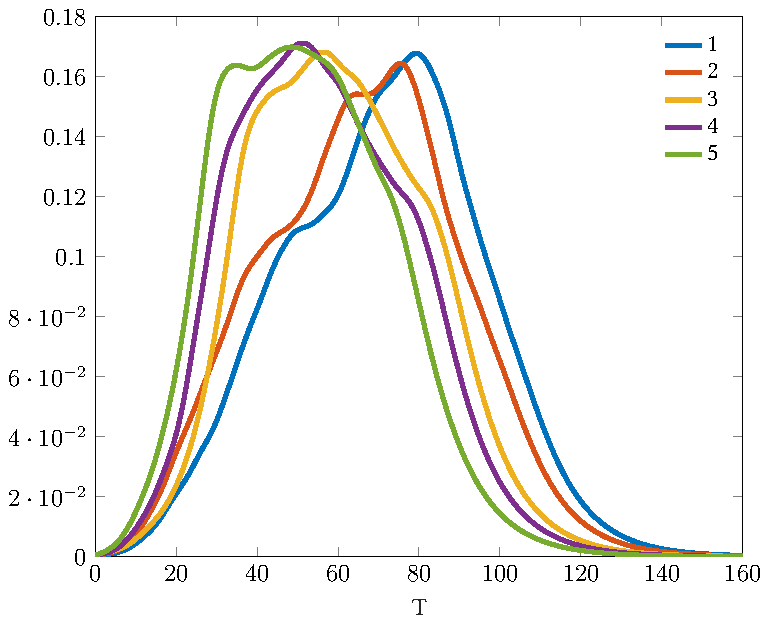
\includegraphics[scale=0.45]{Figure/minnesota_prevalenza}
\caption[Grafico della prevalenza al variare del grado del nodo inizialmente infetto.]{Grafico della prevalenza al variare del grado del nodo inizialmente infetto.\\ Per ottenere i grafici abbiamo risolto numericamente, usando MATLAB, cinque problema di Cauchy ottenuti dal modello chiuso alle coppie.\\
Per le condizioni iniziali abbiamo preso ogni volta un nodo certamente infetto (con grado diverso e tutti gli altri nodi certamente sani).\\
Per la sperimentazione abbiamo utilizzato come parametri $\tau=0.3$ e $\gamma=0.1$}
\label{fig::minnesota_prevalenza}
\end{figure}
